\chapter{Results and Discussion}\label{results}

This chapter summarizes the results of the experiments performed in this research work and described in the previous chapter. The results are presented in the same order of the experiments performed. In this chapter, the results obtained are also discussed and compared with that of obtained using $\theta$RARes model. 

\section{Experiment-1: Models performance on the small corpus}

\paragraph{Word2Vec-ESN Model:} When trained and tested on all the 26 sentences, the model learned the sentences without any errors. But during the cross-validation, the model generalized with $35.09\%$ meaning error and $85.38\%$ sentence error. As illustrated in Table \ref{tab:corpus_45_errors}, it can be seen that with Word2Vec-$\theta$RARes model failed to generalize well on the limited set of 26 constructions. Comparing the performance of the Word2Vec-$\theta$RARes model with the $\theta$RARes model, the generalization errors with Word2Vec-$\theta$RARes model are almost doubled on the same set of 26 constructions. 

It is also important to know that the results of $\theta$RARes model reported in the table \ref{tab:corpus_45_errors} are averaged over 100 reservoir instance of 100 units each \cite{xavier:2013:RT}. Whereas results of Word2Vec-$\theta$RARes are averaged over five reservoir instances of 1000 neurons each. With the small reservoir of 100 neurons, the Word2Vec-$\theta$RARes failed to learn and generalize on the 26 sentences (not reported here).

\begin{table}[H]
\centering
\begin{threeparttable}
\caption[Cross-Validation errors with Word2Vec-$\theta$RARes on limited number of sentences]{Generalization errors in SCL mode on 26 sentences of corpus-45.}
\label{tab:corpus_45_errors}
\rowcolors{2}{gray!25}{white}
\begin{tabular}{llcc}
\toprule
  	 		    		& 		 	&  Word2Vec-$\theta$RARes 	& $\theta$RARes \\
\midrule                 
\textbf{Meaning Error}	& mean 		& 35.09  					& 14.83  \\
						& std. 		& 05.89 					& 02.59  \\
\textbf{Sentence Error}	& mean 		& 85.38  					& 42.73 \\
						& std. 		& 07.88 					& 07.19 \\
\bottomrule
\end{tabular}
\begin{tablenotes}
\small
\item 
LoO cross-calidation errors with both Word2Vec-$\theta$RARes model and $\theta$RARes model (shown in \%). Mean and std. is average and standard deviation of errors over several model instances.
\end{tablenotes}
\end{threeparttable}
\end{table}

\paragraph{Word2Vec-ESN classifier:} As illustrated in Table \ref{tab:corpus_45_scores}, the Word2Vec-ESN classifier learned the 26 sentences resulting in F1-Score of $95.69\%$. While testing using LoO cross-validation method the model resulted into low F1-Score of $68.53\%$. The high difference in F1-Score during training and testing points toward the limited generalization on unseen sentences. 

\begin{table}[H]
\centering
\begin{threeparttable}
\caption[Generalization score with Word2Vec-ESN classifier on limited number of sentences.]{Classification score of model Word2Vec-ESN classifier on 26 sentences from corpus-45.}
\label{tab:corpus_45_scores}
\rowcolors{2}{gray!25}{white}
\begin{tabular}{llccc}
\toprule
  	 			& 		 	&  Precision 		& Recall	& F1-Score\\
\midrule                
\textbf{train}	& mean 		& 94.92  			& 96.54 	& 95.68  \\
				& std. 		& 00.27 			& 00.74  	& 00.46  \\
\textbf{test}	& mean 		& 69.87  			& 71.29  	& 68.53 \\
				& std. 		& 02.36 			& 01.37 	& 01.80  \\
\bottomrule
\end{tabular}
\begin{tablenotes}
\small
\item 
LoO classification scores of Word2Vec-ESN classifier(shown in \%). Mean and std. is average and standard deviation of classification scores over several model instances.
\end{tablenotes}
\end{threeparttable}
\end{table}


\section{Experiment-2: Generalization Capabilities} \label{exp-2}

\paragraph{Word2Vec-$\theta$RARes model:} When the model was initially trained and tested on all the 462 sentences of corpus-462, it learned the sentences with $0.55\%$ meaning error and $1.64\%$ sentence error in the SCL mode and $0.16\%$ meaning error and $0.52\%$ sentence error in the SFL mode. Using the 10-fold cross-validation, the model generalized to $8.68\% (\pm 1.01\%) $ meaning error and $24.09\% (\pm 2.38\%)$ sentence error in the SCL mode. Whereas in the SFL mode the optimal meaning and sentence error were observed as $8.88\% (\pm 0.14\%)$ and $25.17\% (\pm 0.01\%)$ respectively.

As illustrated in Table \ref{tab:corpus-462_errors}, one can see that while training both the Word2Vec-$\theta$RARes and $\theta$RARes model learned all the sentences thoroughly (less than $ 1\% $ error rates) in SCL and  SFL mode. Comparing the performance of both the model during testing, we can see an improvement of $8.04 \%$ sentence error in SCL mode with Word2Vec-$\theta$RARes model, whereas the meaning error dropped by $1.25 \%$. However, considering the standard deviation, we can also say that the meaning error remained almost equivalent in both the Word2Vec-$\theta$RARes and $\theta$RARes model. In SFL mode, both the meaning and sentence errors remained nearly equal for both the models. It can also be observed that with Word2Vec-$\theta$RARes model, the performance of the model is improved mainly in SCL mode as compared to SFL mode, whereas it is vice-versa in $\theta$RARes model. 

%NOTE: 08/09/2016 results are copied after the simulation and are final, no need to change.
\begin{table}[htbp]
\centering
\begin{threeparttable}
\caption{Mean and standard deviation of meaning and sentence error on train and test set of coprus-462 in different learning modes.}
\label{tab:corpus-462_errors}
\rowcolors{2}{white}{gray!25}
\begin{tabular}{llrrrrrrrr}
  \toprule
  \hiderowcolors   
  &  & \multicolumn{4}{c}{Word2Vec-$\theta$RARes} & \multicolumn{4}{c}{$\theta$RARes} \\
  \cmidrule(lr){3-6}   \cmidrule(lr){7-10}
  
  &  & \multicolumn{2}{c}{Corpus 462} & \multicolumn{2}{c}{462 scrambled} & \multicolumn{2}{c}{Corpus-462} & \multicolumn{2}{c}{462 scrambled} \\
  \cmidrule(lr){3-4} \cmidrule(lr){5-6}  \cmidrule(lr){7-8} \cmidrule(lr){9-10}  
  
  
   						& 		& ME 	& SE 		& ME 	 & SE 		& ME 	& SE		& ME 	& SE 		\\
  \midrule
  \showrowcolors
  \textbf{SCL\ train} 	& mean 	& 0.55 & 1.64  		& 6.68  & 26.80	 	& 0.12 & 1.21 	& 4.81  & 20.43	\\
   			    		& std 	& 0.06 & 0.12 		& 0.67  & 1.64 		& 0.03 & 0.30 	& 0.30  & 1.25	\\
   			    		
  \textbf{SCL\ test} 	& mean  & 8.68 & 24.09 		& 70.15 & 99.26 	& 7.43 & 32.13 	& 74.15 & 99.89	\\
  			   			& std  	& 1.01 & 2.38 		& 1.24  & 0.29  	& 0.52 & 1.35 	& 0.80  & 0.15	\\
  			   			
  \textbf{SFL\ train} 	& mean 	& 0.16 & 0.52 		& 9.38  & 35.58 	& 0.00 & 0.00 	& 0.00  & 0.00	\\
  				 		& std 	& 0.09 & 0.25 		& 0.69  & 3.40 		& 0.00 & 0.00 	& 0.00  & 0.00	\\
  				 		
  \textbf{SFL\ test}	& mean  & 8.88 & 25.17 		& 67.87 & 99.26 	& 9.18 & 24.37 	& 73.39 & 99.91	\\
  			  			& std 	& 0.14 & 0.01		& 0.10  & 0.33  	& 0.57 & 1.19 	& 0.96  & 0.11	\\
  \bottomrule
\end{tabular}
\begin{tablenotes}
\small
\item 
Meaning (ME) and Sentence error (SE) in different learning modes with Word2Vec-$\theta$RARes model using distributed word embeddings and $\theta$RARes model \cite{xavier:2013:RT} which uses grammatical form and localist representation of words of sentences. The errors are given in percentage with two decimal precision. SCL: Sentence Continuous Learning; SFL: Sentence Final Learning; std: standard deviations. Simulations were done with 5 model instances with the reservoir of 1000 neurons.
\end{tablenotes}
\end{threeparttable}
\end{table}


\paragraph{Word2Vec-ESN classifier:} 

Table \ref{tab:corpus-462-scores}, illustrates the training and cross-validation classification scores of simulations performed with the Word2Vec-ESN classifier in both the configurations as described in Experiment-2 (see section \ref{exp-2}). In configuration-1, the model when trained and tested on all the 462 sentences of corpus-462, the model learned to label the argument-predicate pairs in the sentences with the Precision (Pr), Recall (Re) and F1-Score (F1) of $97.46 \%$, $92.29 \%$, $94.65 \%$ respectively. When tested using 10-fold cross validation for generalization, the model genralized with Pr = $96.76 \% $, Re = $91.78 \%$ and F1 = $93.99 \%$. Notice the marginal difference between the training and cross validation scores, indicating that the Word2Vec-ESN classifier in configuration-1 is generalizing well on untrained sentences and is not overfitting.

In configuration-2, where the sentences are transformed to GF and localist word representations are used as an input to ESN, the model learned the sentences with Pr = $61.96 \% (\pm 0.07\%)$, Re = $67.69 \% (\pm 0.29\%)$, F1 = $63.55 \% (\pm 0.17\%)$ during training. With 10-fold cross-validation the model generalized with Pr = $61.91 \% (\pm 0.07\%)$, Re = $68.20 \% (\pm 0.46\%)$ and F1 = $63.71 \% (\pm 0.22\%)$. It can be noticed that the Word2Vec-ESN classifier in configuration-2 did not perform well in comparision with configuration-1. Both the training and testing scores are much lower when compared to scores of configuration-1.


\begin{table}
\centering
\begin{threeparttable}
\caption{Classification scores produced by Word2Vec-ESN classifier on unscrambled and scrambled corpus-462 in two configurations.}
\label{tab:corpus-462-scores}
\rowcolors{2}{white}{gray!25}
\begin{tabular}{llllll}
  \toprule
  \hiderowcolors   
  &  & \multicolumn{2}{c}{Configuration-1} & \multicolumn{2}{c}{Configuration-2} \\
  \cmidrule(lr){3-4}    \cmidrule(lr){5-6} 
  &  & \multicolumn{1}{c}{coprus-462} & \multicolumn{1}{c}{462 scrambled} & \multicolumn{1}{c}{coprus-462} & \multicolumn{1}{c}{462 scrambled} \\
   			
  \midrule
  \showrowcolors
  \textbf{Precision} 	& test 		& 96.76 ($\pm$ 0.08) & 95.72 ($\pm$ 0.15)	& 61.91 ($\pm$ 0.07) & 16.71 ($\pm$ 0.64) 	\\
   			    	  	& train 	& 97.46 ($\pm$ 0.00) & 96.96 ($\pm$ 0.13)	& 61.96 ($\pm$ 0.07) & 57.24 ($\pm$ 7.90)	\\
   			    		
  \textbf{Recall} 		& test  	& 91.78 ($\pm$ 0.08) & 89.75 ($\pm$ 0.11)	& 68.20 ($\pm$ 0.46) & 20.01 ($\pm$ 0.02) 	\\
  			   			& train 	& 92.29 ($\pm$ 0.22) & 90.40 ($\pm$ 0.05)	& 67.69 ($\pm$ 0.29) & 20.17 ($\pm$ 0.04)	\\
  			   			
  \textbf{F1-Score} 	& test 		& 93.99 ($\pm$ 0.09) & 92.28 ($\pm$ 0.12) 	& 63.71 ($\pm$ 0.22) & 17.49 ($\pm$ 0.05)	\\
  				 		& train 	& 94.65 ($\pm$ 0.00) & 93.24 ($\pm$ 0.08)	& 63.55 ($\pm$ 0.17) & 17.74 ($\pm$ 0.08)	\\  				 		
  
  \bottomrule
\end{tabular}
\begin{tablenotes}
\small
\item 
{\small Classification scores (in  $\%$) of Word2Vec-ESN classifier during training and testing condition. Configuration-1: raw sentences are processed, and distributed vectors of the argument-predicate pair are input to ESN. Configuration-2: Sentences transformed to grammatical form and localist word vectors are input to ESN. Simulations were done with five instances of Word2Vec-ESN classifier each with a reservoir of 1000 neurons.}
\end{tablenotes}
\end{threeparttable}
\end{table}

% CONFUSION MATRIX
\begin{figure}[hbtp]
\centering
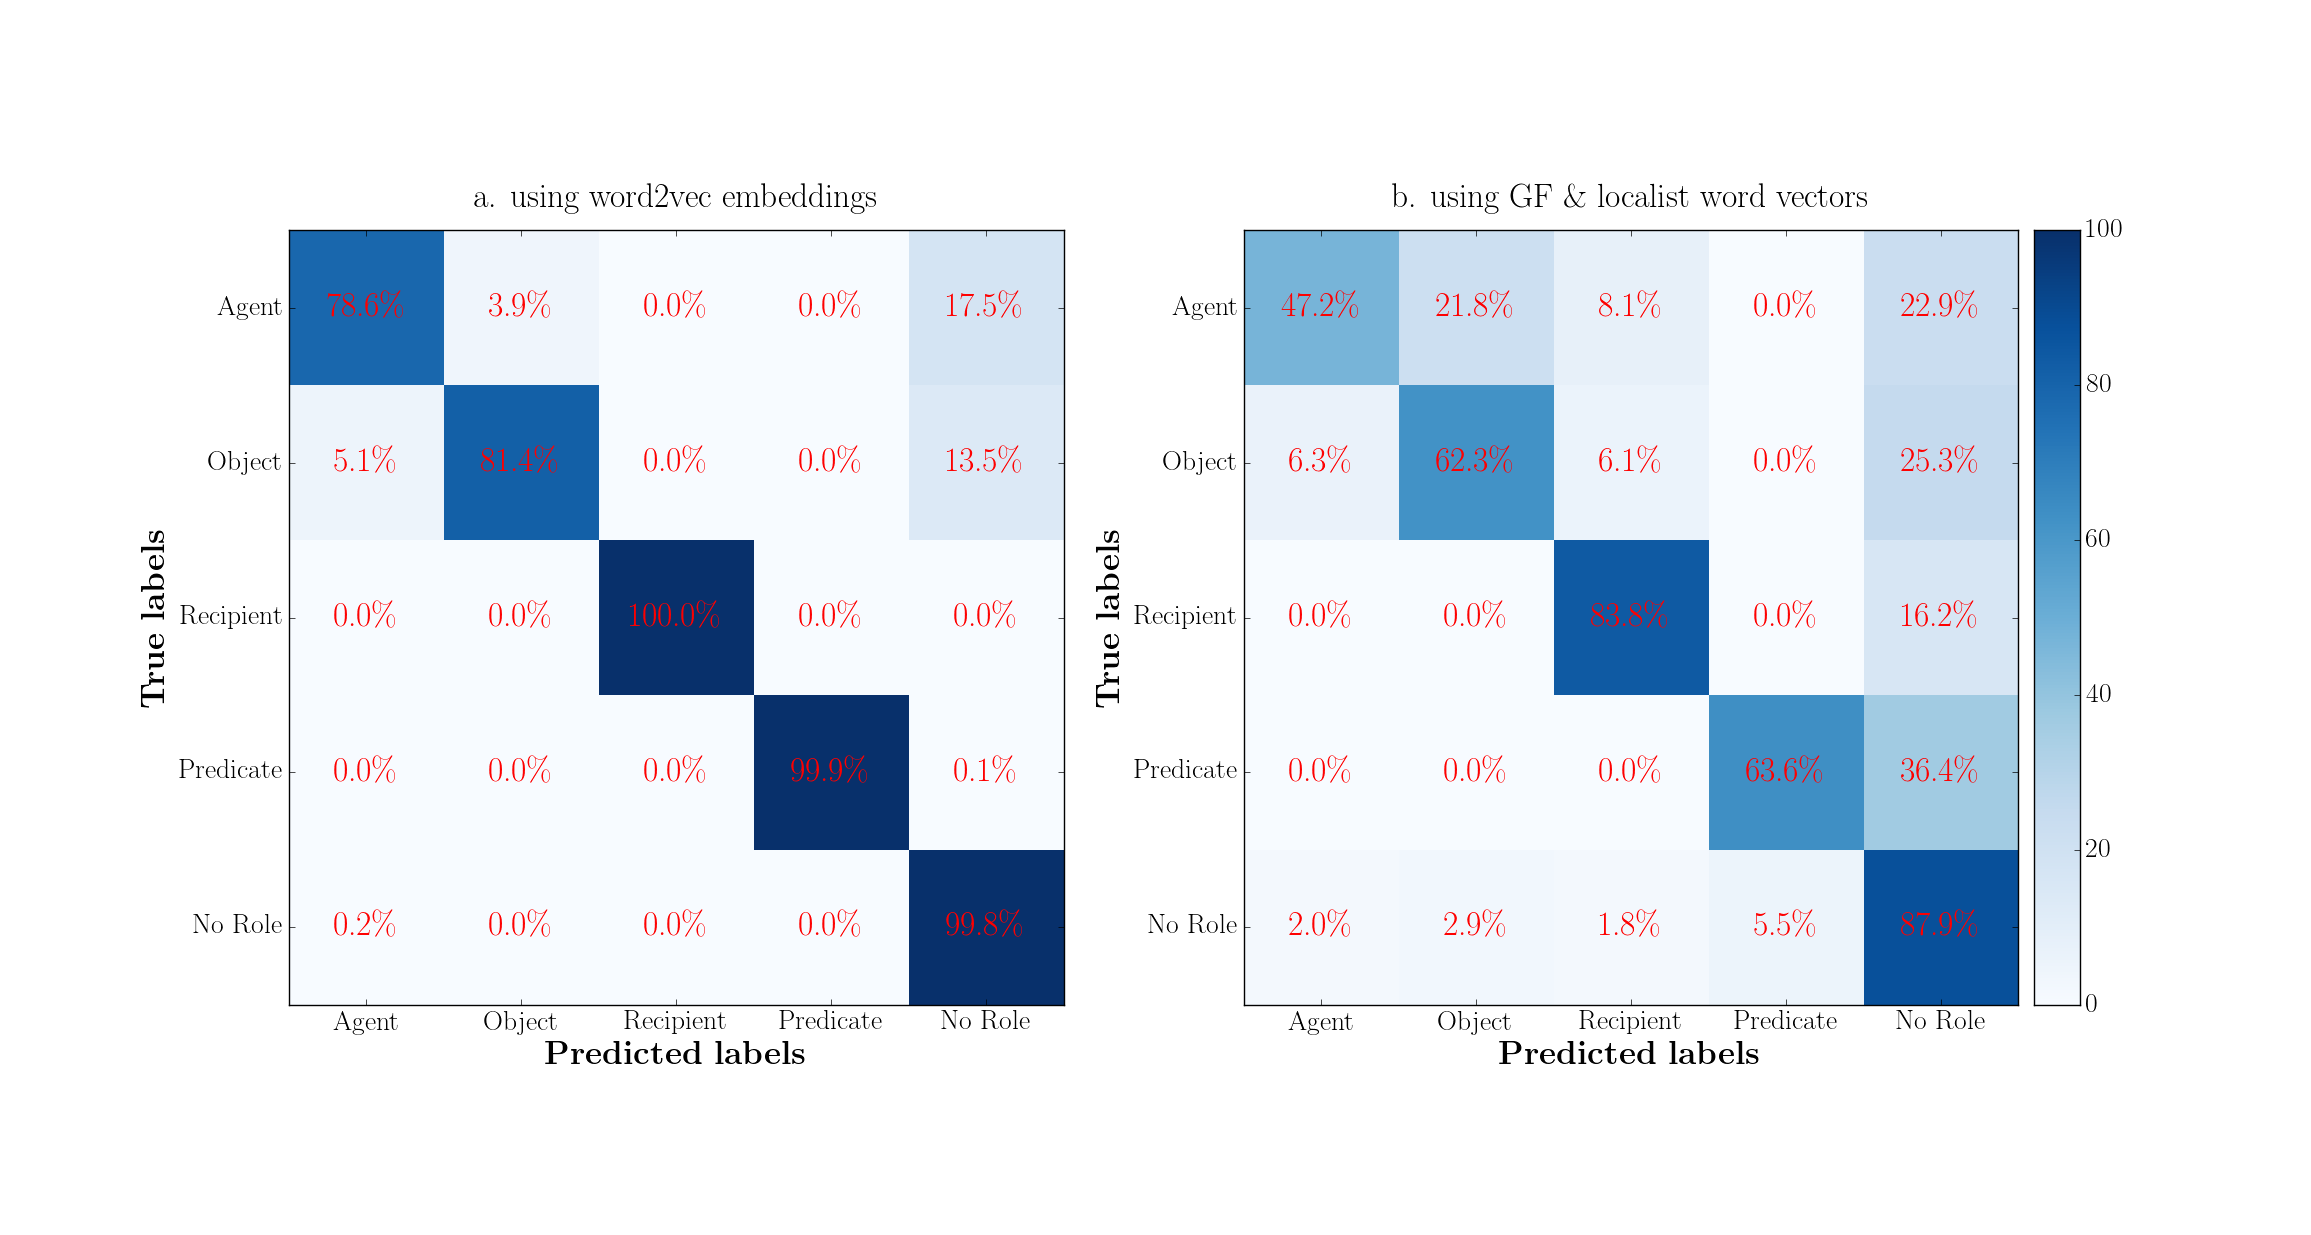
\includegraphics[width=1.0\linewidth]{confusion_matrix}
\caption[Normalized confusion matrix on corpus 462 with Word2Vec-ESN classifier] {\textbf{Normalized confusion matrix with Word2Vec-ESN classifier in configuration-1 and configuration-2:}{\small The confusion matrix with true roles (in rows) and predicted roles (in columns). The top-left to bottom-right diagonal shows the percentage of words whose roles are predicted correctly. Everything other than this diagonal represents the incorrect prediction of roles. Configuration-1: raw sentences processed by Word2Vec-ESN classifier and word2vec word vectors are input to ESN. Configuration-2: Sentences transformed to grammatical form and localist word vectors are input to ESN. The results were obtained with reservoir of 1000 neurons and 10 fold-cross validation.}}
\label{fig:confusion_matrix}
\end{figure}

% CONFUSION MATRIX SCRAMBLED
\begin{figure}[hbtp]
\centering
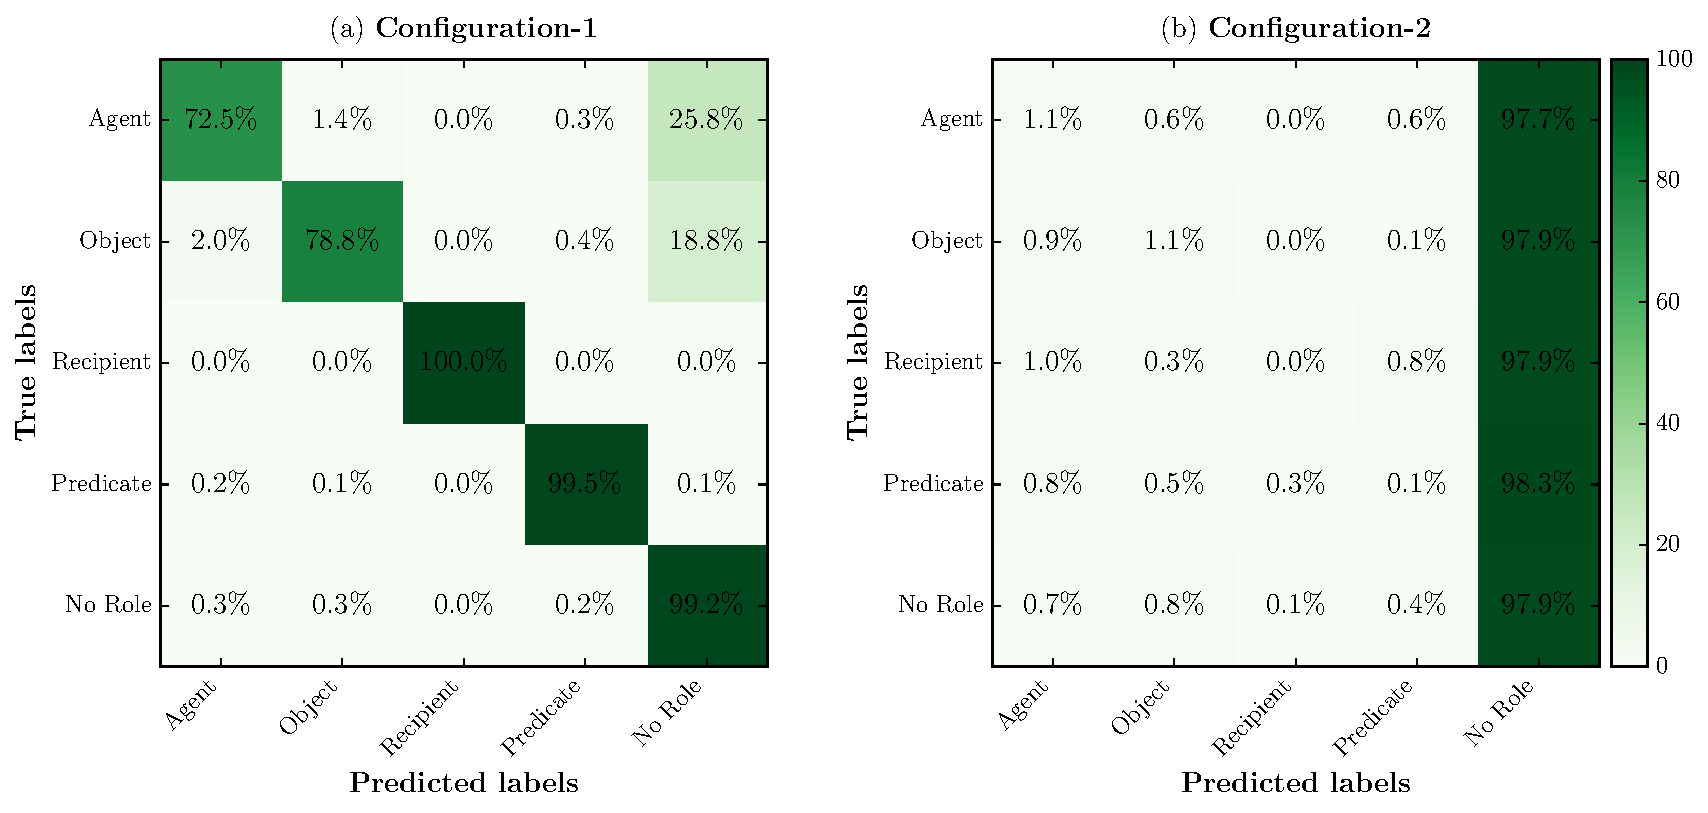
\includegraphics[width=1.0\linewidth]{confusion_matrix_shuffle}
\caption[Normalized confusion matrix on scrambled corpus 462 with Word2Vec-ESN classifier] {\textbf{Normalized confusion matrix with the Word2Vec-ESN classifier on scrambled corpus-462:} The confusion matrix with true roles (in rows) and predicted roles (in columns). The top-left to bottom-right diagonal shows the percentage of words whose roles are predicted correctly. Everything other than this diagonal represents the incorrect prediction of roles. Configuration-1: raw sentences processed by the Word2Vec-ESN classifier and word2vec word vectors are input to ESN. Configuration-2: Sentences transformed to grammatical form and localist word vectors are input to ESN. The results were obtained with reservoir of 1000 neurons and 10 fold-cross validation.}
\label{fig:confusion_matrix_shuffle}
\end{figure}

Figure \ref{fig:confusion_matrix} shows the confusion matrix, plotted using cross-validation results of the Word2Vec-ESN classifier in configuration-1 and configuration-2 (see section \ref{exp-2}). The corresponding classification scores of individual roles produced by Word2Vec-ESN classifier during 10-fold cross-validation in both the configuration are also reported in Table\ref{tab:classsification-scores-21}.

As seen in the confusion matrix (see fig. \ref{fig:confusion_matrix}), when using the distributed vectors of argument-predicate pair as an input to ESN (i.e. configuration-1), the model predicted the words with the role `Recipient', `Predicate' and `No Roles' almost without making any errors. The model predicted $78.6 \%$ of the words with the role `Agent' correctly, whereas $3.9 \%$ and $17.5 \%$ of the words with the role `Agent' were incorrectly predicted as `Object' and `No Role' respectively. Similarly, $81.4 \%$ of the words with the role `Object' were correctly classified, whereas $ 5.1 \%$ of the words with actual roles as `Object' were misclassified as `Agent' and $13.5 \%$ as `No Role'. On the other hand, only $0.2 \%$ the words with the actual role `No Role' were wrongly predicted as 'Agent'. 

Using the sentences in GF along with localist word vectors of the argument-predicate pair, as an input to ESN, the roles `Recipient' and `No Role' were correctly predicted with least errors of $16.2 \%$ and $12.1 \%$. The Word2Vec-ESN classifier wrongly predicted all the roles as `No Role', where the `Predicate' being the highest role to be misclassified as `No Role' ($36.4 \%$). The model seems to be confused with the words having roles `Agent' and `Object'. $21.8 \%$ of the words with the role `Agent' were incorrectly predicted as `Object', whereas $6.3 \%$ of words with the actual role as `Object' were misclassified as `Agent'. Also, the words with the roles `Agent' and `Object' were confused with the role `Recipient'. $8.1 \%$ of the words with the role `Agent' were wrongly predicted as `Recipient' and $6.1 \%$ of the words with the role `Object' were incorrectly predicted as `Recipient'. 

While comparing the predictions made by the Word2Vec-ESN classifier in both the configurations, it was observed that the roles `Agent' and `Object' made the most number of error in predictions as compared to other roles. In configuration-2, the roles `Agent' and `Object' were wrongly predicted as `Recipient', whereas in configuration-1, this misprediction does not exist. Comparing the false predictions made by the Word2Vec-ESN classifier in both the configurations, it was observed that in configuration-1, the incorrect predictions were comparatively less. In configuration-1, all the words with roles `Recipient', `Predicate' and `No Role' were predicted almost without any errors whereas, in configuration-2, the Word2Vec-ESN classifier misclassified these roles respectively by $16.2 \%$, $36.4\%$, and $12.1 \%$.


%NOTE: 08/09/2016 results are copied after the simulation and are final, no need to change.
\begin{table}[h]
\centering
\begin{threeparttable}
\caption{Training and testing classification scores for individual roles when using Word2Vec-ESN classifier in two different configurations.}
\label{tab:classsification-scores-21}
\rowcolors{2}{gray!25}{white}
\begin{tabularx}{\textwidth}{@{}llYYYYYYY@{}}
\hiderowcolors
\toprule
  &  & \multicolumn{3}{c}{Configuration-1} & \multicolumn{3}{c}{Configuration-2}& \\  
\cmidrule(lr){3-5}   \cmidrule(lr){6-8}
   
Role 				& 			& Pr   & Re  & F1 		& Pr  &  Re & F1 		&  Support  \\
\showrowcolors
\midrule
               
\textbf{Agent}		&test 		& 0.92 & 0.79 & 0.85 	& 0.63 & 0.47 & 0.54	& 888  \\
					&train  	& 0.94 & 0.80 & 0.86 	& 0.64 & 0.46 & 0.53	& 892  \\
\textbf{Object}		&test 		& 0.95 & 0.81 & 0.88 	& 0.51 & 0.62 & 0.56	& 791  \\
					&train  	& 0.96 & 0.82 & 0.88 	& 0.51 & 0.61 & 0.56	& 794  \\
\textbf{Recipient}	&test 		& 1.00 & 1.00 & 1.00 	& 0.52 & 0.84 & 0.64	& 382  \\
					&train  	& 1.00 & 1.00 & 1.00 	& 0.52 & 0.83 & 0.64	& 384  \\
\textbf{Predicate}	&test		& 1.00 & 1.00 & 1.00 	& 0.51 & 0.64 & 0.57	& 888  \\
					&train  	& 1.00 & 1.00 & 1.00 	& 0.51 & 0.64 & 0.57	& 892   \\
\textbf{No Role}	&test 		& 0.97 & 1.00 & 0.99 	& 0.92 & 0.88 & 0.90	& 9776  \\
					&train  	& 0.97 & 1.00 & 0.99 	& 0.91 & 0.88 & 0.90	& 9823  \\
\bottomrule
\end{tabularx}
\begin{tablenotes}
\small
\item Training and cross-validation classification scores (precision upto 2 decimals) for each output roles predicted by the Word2Vec-ESN classifier in two configuration. Support for each role: actual number of instances, is also shown in last column. Simulation condition: 1000 reservoir neurons, 10-fold cross-validation.
\end{tablenotes}
\end{threeparttable}
\end{table}

\section{Experiment-3: Effect of Corpus structure} 

\paragraph{Word2Vec-$\theta$RARes model:}As illustrated in Table \ref{tab:corpus-462_errors}, it was observed that when using the scrambled corpus as an input to the Word2Vec-$\theta$RARes model, the model learned with low error rates of $ME = 6.68 \%$ and $SE = 26.80 \%$ in SCL mode. While testing, the model generalized with cross-validation error rates of $ME = 70.15 \% $ and $SE = 99.26 \%$. Similarly, in SFL mode the model learned with low error rates of $ME = 9.38 \%$ and $SE = 35.58 \%$  but during cross-validation high error rates of $ME = 67.87 \%$ and $SE = 99.26 \% $ was observed. Notice that the model learned the scrambled corpus with low error rates while training but during the cross-validation resulted into high error rates.

\paragraph{Word2Vec-ESN classifier:} Table \ref{tab:corpus-462-scores} illustrates the effect of scrambled corpus on the Word2Vec-ESN classifier. It can be seen that in the configuration-1, the classification scores remained almost equivalent to that obtained with the unscrambled corpus. Whereas in the configuration-2, the Word2Vec-ESN classifier failed to learn and generalize as well. The classification score during training and testing are lower than that obtained with unscrambled corpus. 

Figure \ref{fig:confusion_matrix_shuffle} shows the confusion matrix obtained when using the scrambled corpus as an input to Word2Vec-ESN classifier. It was observed that in configuration-1, the Word2Vec-ESN classifier classifies the argument-predicate pair to the respective roles with high classification scores whereas, in configuration-2, it fails to do so. Comparing the confusion matrix obtained when using unscrambled corpus-462 (see fig. \ref{fig:confusion_matrix}) and scrambled corpus-462 (see fig. \ref{fig:confusion_matrix_shuffle}) it is clearly visible that in configuration-1, the classification scores for each roles is negligibly affected. Whereas in configuration-2, the classification scores of individual roles dropped heavily.

\section{Experiment-4: Effect of Reservoir size}

\paragraph{Word2Vec-$\theta$RARes model: } Figure \ref{fig:reservoir_size_1} shows the effect of reservoir size on the cross-validation errors rates (i.e. meaning and sentence error). The meaning and sentence error continuously drops with the increase in reservoir size from 90 to 1098 in both the learning modes.  As the reservoir size is further increased from 1098, the meaning error in the SFL mode slightly increases ($\approx 1\%$), whereas it remains unchanged in the SCL mode. On the other hand, the sentence error in the SFL mode slightly increases whereas in the SCL mode it is negligibly dropped when the reservoir size is further increased from 1776 to 2882 and remains stable after that. Overall, it was observed that both the meaning and sentence cross-validation error rates reduce with increase in reservoir size but asymptotes when the reservoir size is above 1000 on the corpus-462.

\begin{figure}[hbtp]
\centering
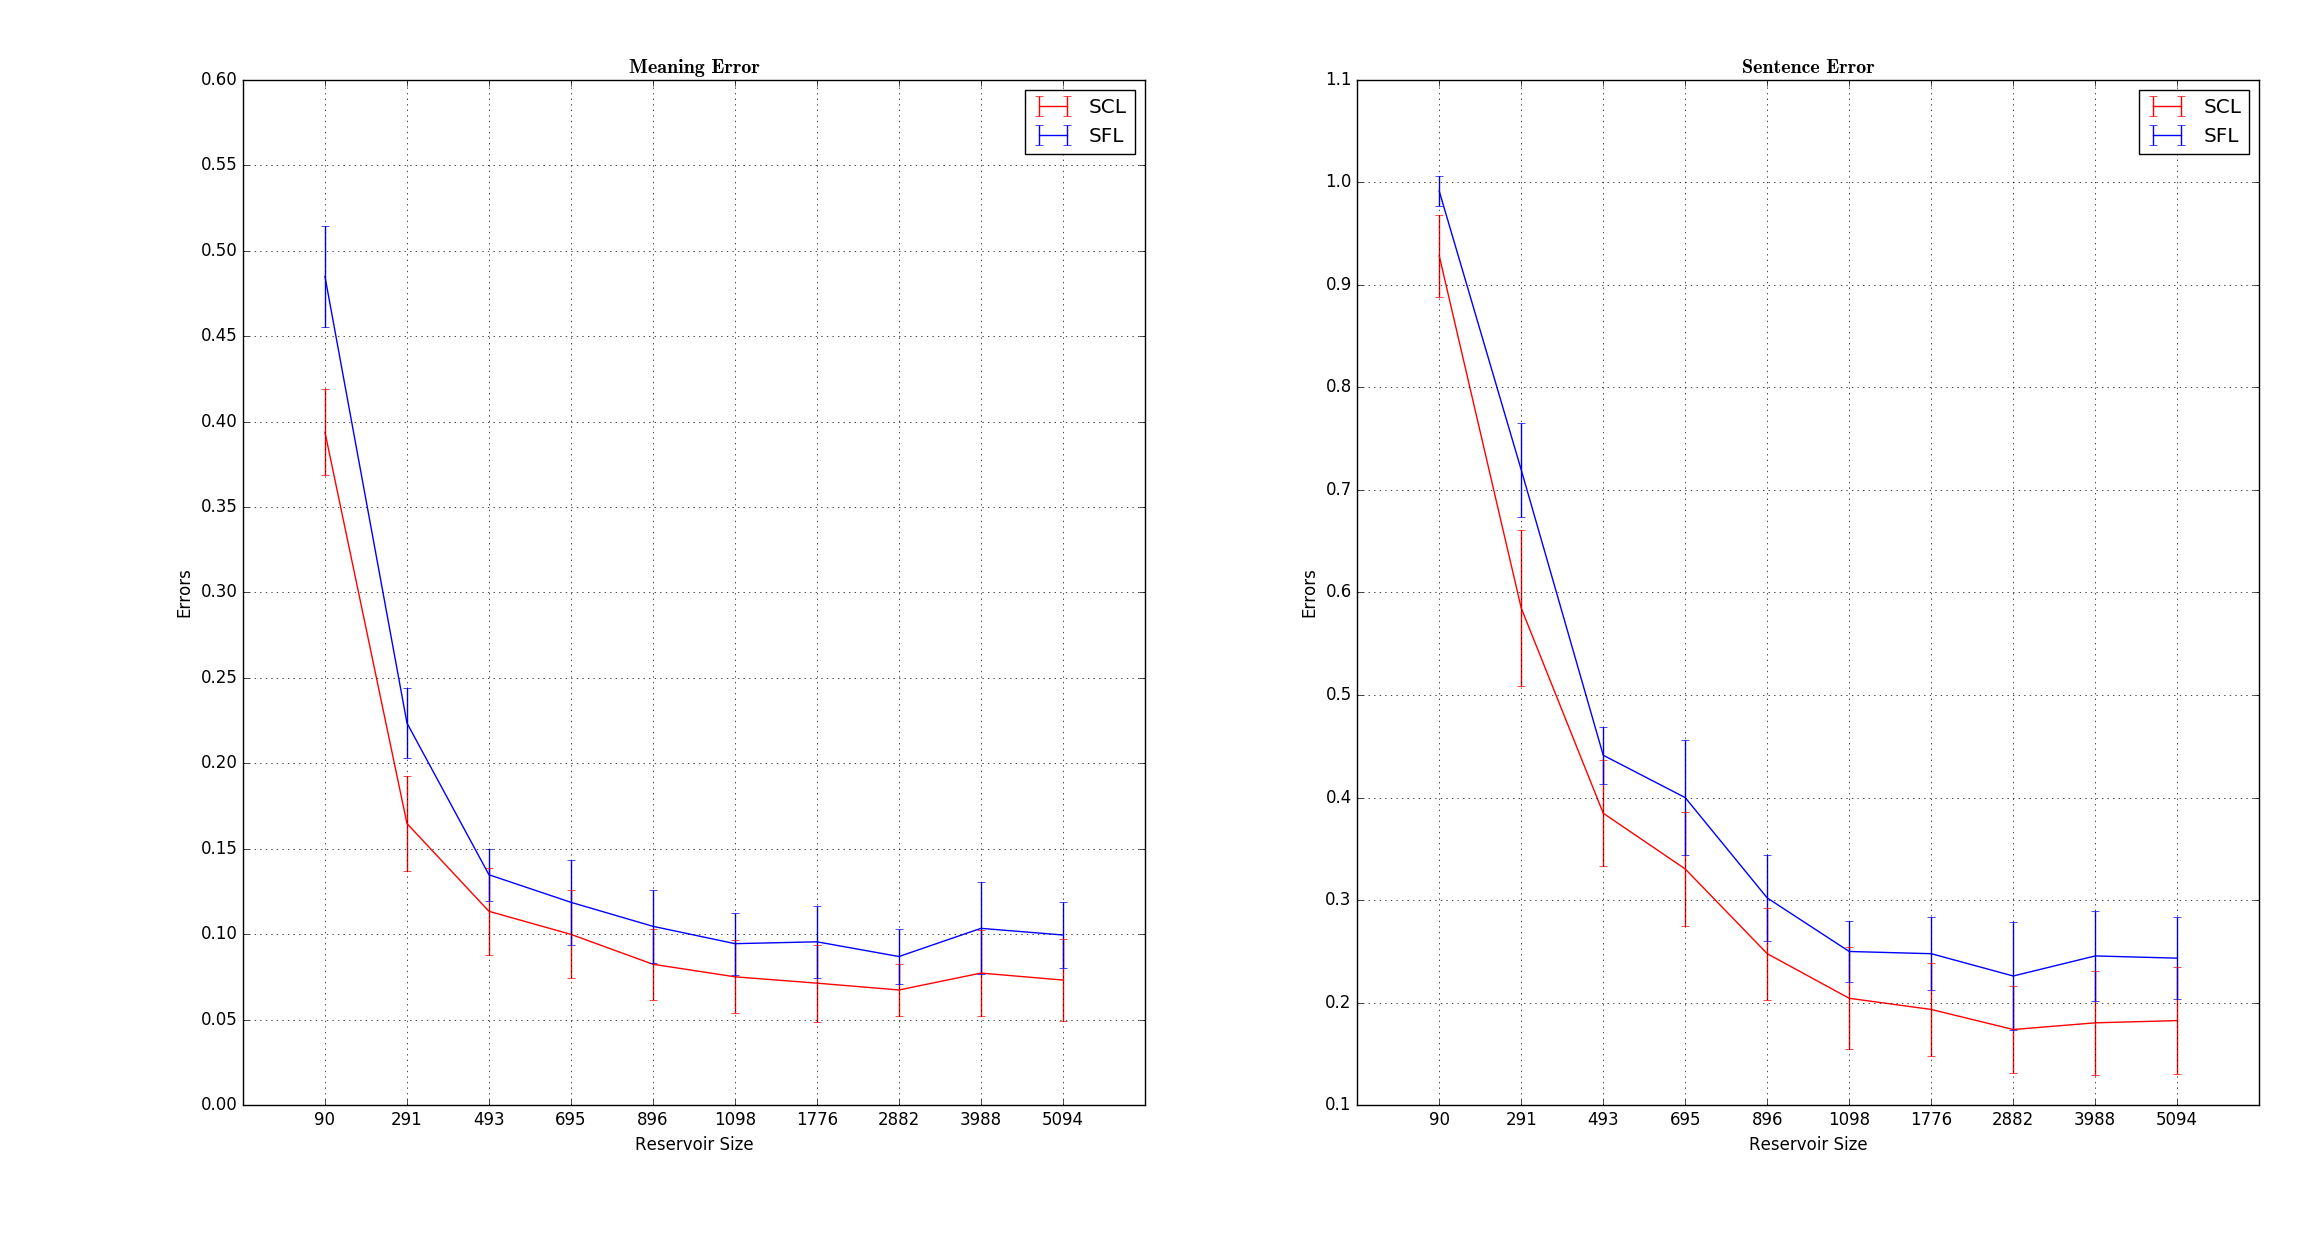
\includegraphics[width=1.0\linewidth]{reservoir_size_1}
\caption[Effect of reservoir size on Word2Vec-$\theta$RARes model]{Effect of reservoir size on cross-validation errors of Word2Vec-$\theta$RARes model.}
\label{fig:reservoir_size_1}
\end{figure}

\begin{figure}[hbtp]
\centering
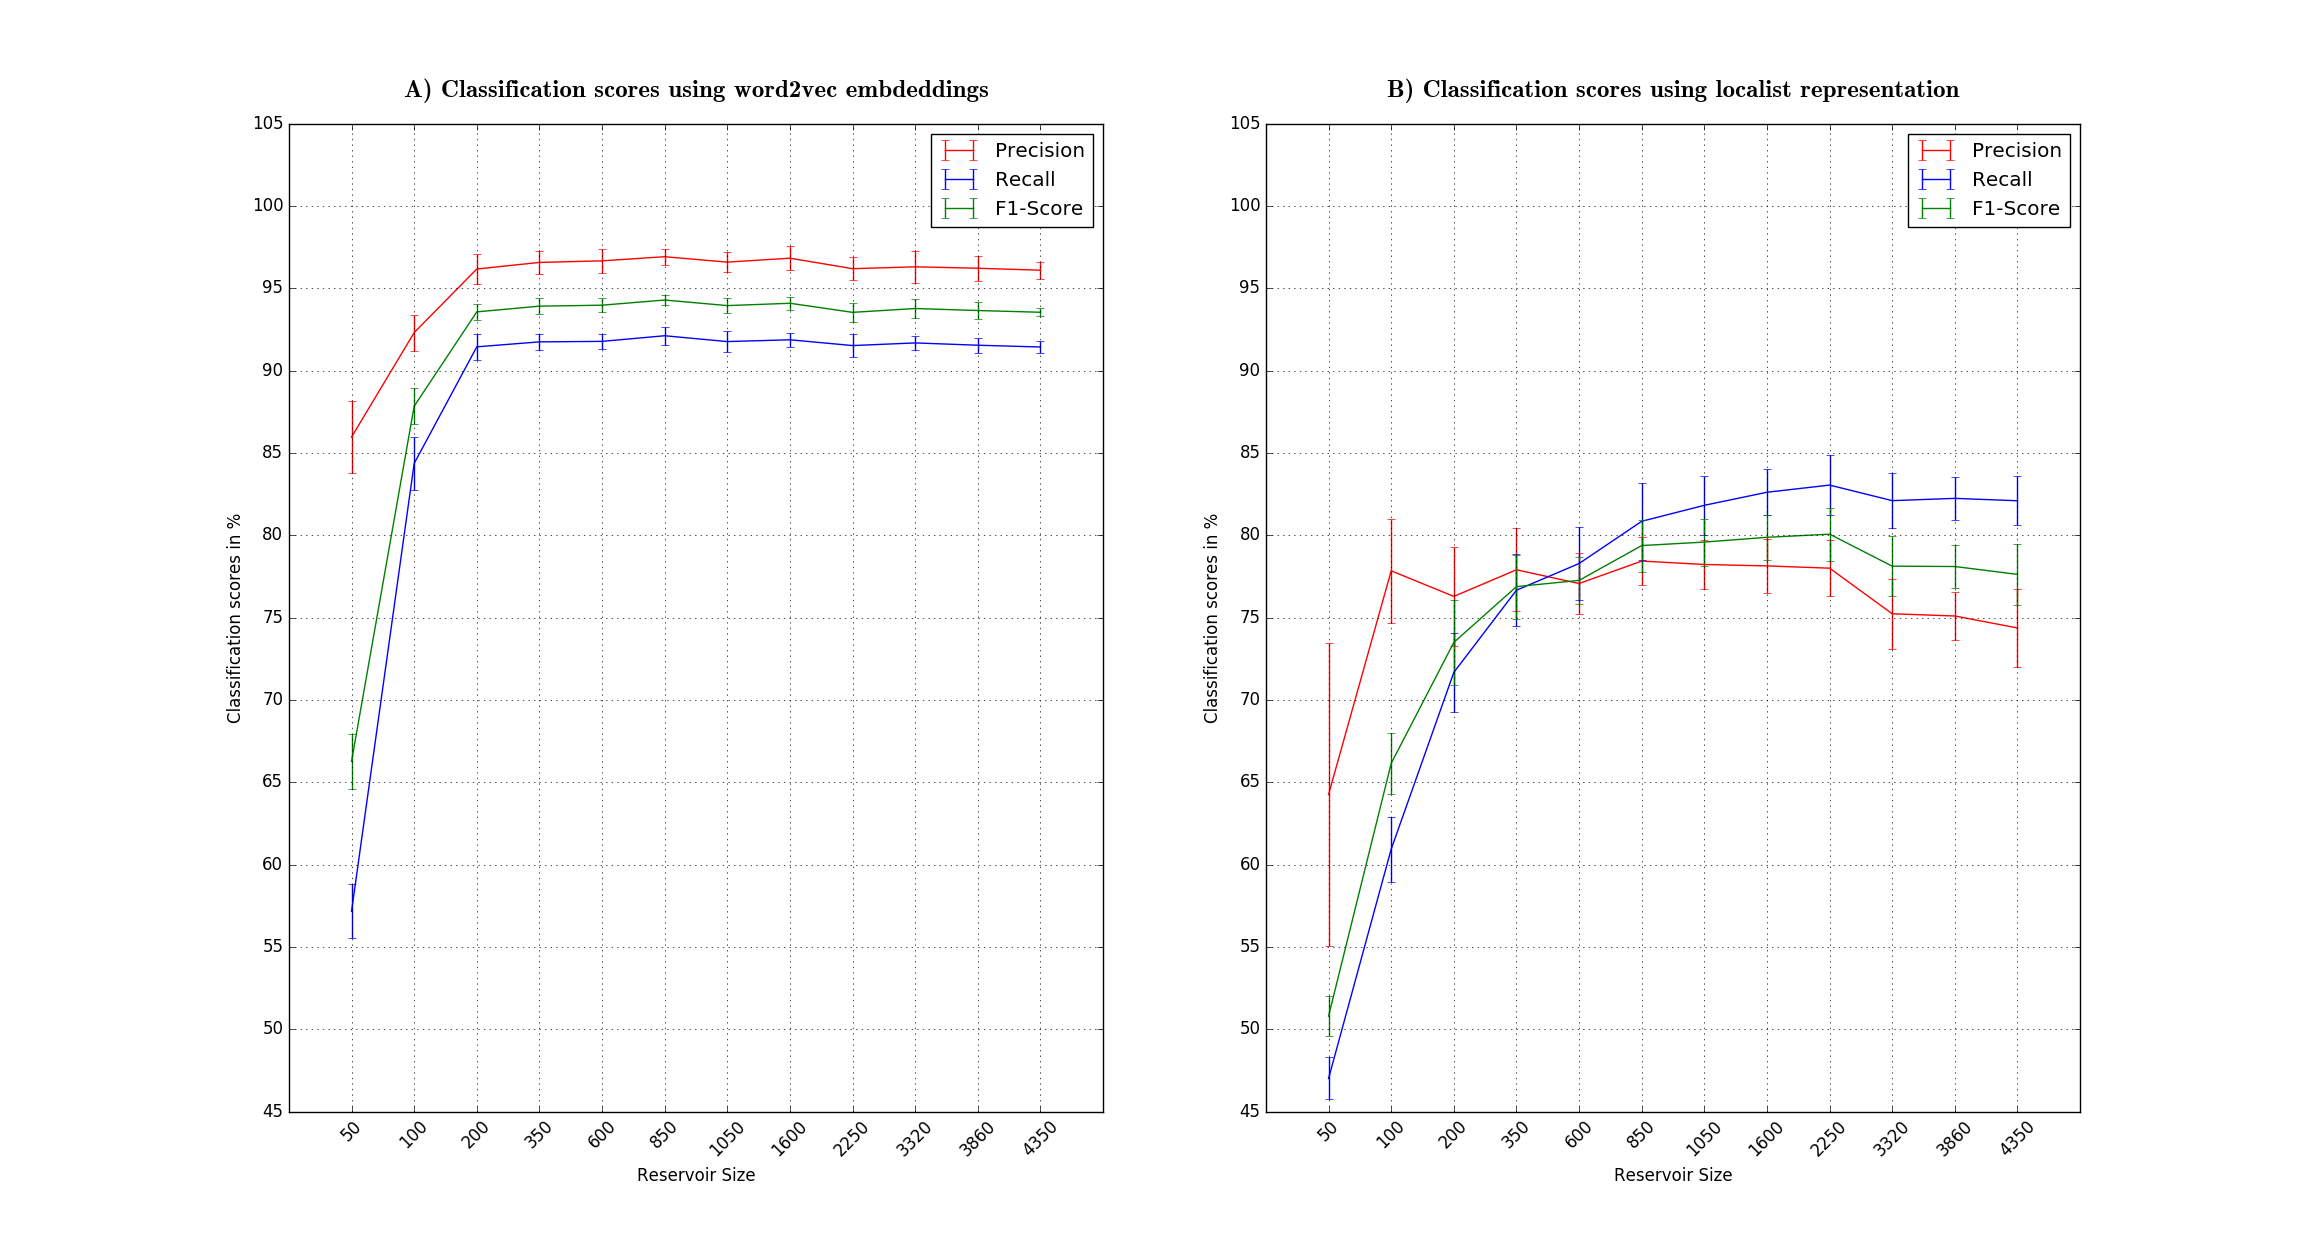
\includegraphics[width=1.0\linewidth]{reservoir_size_2}
\caption[Effect of reservoir size on Word2Vec-ESN classifier]{Effect of reservoir size on classification scores of Word2Vec-ESN classifier}
\label{fig:reservoir_size_2}
\end{figure}

\paragraph{Word2Vec-ESN classifier: } Figure \ref{fig:reservoir_size_2} shows the change in classification scores of the Word2Vec-ESN classifier with the increase in reservoir size. It can be observed that when using the distributed word vectors (i.e. configuration-1) the classification scores sharply increases when the reservoir size is increased from 50 neurons to 250 neurons. As the reservoir size is further increased from 250 neurons, the classification scores remain stable with the neglible drop of scores. Whereas, in configuration-2 (i.e. when using GF and Localist representation) the classification scores also improves, with the increase in reservoir size from 50 to 250 neurons. As the reservoir size is further increased from 250 neurons, the recall is improved whereas the precision remains almost flat with negligible improvement. The F1-Score is harmonic mean of precision and recall; it was also slightly increased. Even the highest F1-Score of Word2Vec-ESN classifier observed at reservoir size 4500 in configuration-2, is much lower than that of observed at reservoir size 100 ($\approx 29 \%$ ) in configuration-1.

\section{Experiment-5: Scalability of the model}

Figure \ref{fig:corpus_size_1} shows the cross-validation errors rates with respect to corpus size on the Word2Vec-$\theta$RARes model. It can be observed that with increase in corpus size from $6 \%$  to $50 \%$, the meaning error sharply drops from some $12.18 \% (\pm 0.19 \%)$ to $2.96 \%(\pm 0.04\%)$ in the SCL mode and from $11.96\%(\pm 0.35\%)$ to $4.17 \%(\pm 0.11\%)$ in the SFL mode. Similarly, the sentence error also decreases from $54.84 \%(\pm 0.52\%)$ to $17.25 \%(\pm 0.39\%)$ in SCL and from $54.14 \%(\pm 1.28\%)$ to $22.41 \% (\pm 0.57\%)$ in the SFL mode. When the sub-corpora size is $75\%$, where the model was trained only on $37.5\%$ of corpora size, the model already generalized with $2.72 \%(\pm 0.03\%)$ meaning error and $15.98 \% (\pm 0.30\%)$ sentence error in the SCL mode and with $3.95 \%(\pm 0.11\%)$ meaning error and $21.33 \%(\pm 0.64\%)$ sentence error in the SFL mode.Although the error rates gradually drops when the corpus size is further increased from $25\%$ to $100\%$ but the improvement rate of errors is very less. Thus the further increase in corpus size will not have much effect on cross-validation error.

\begin{figure}[hbtp]
\centering
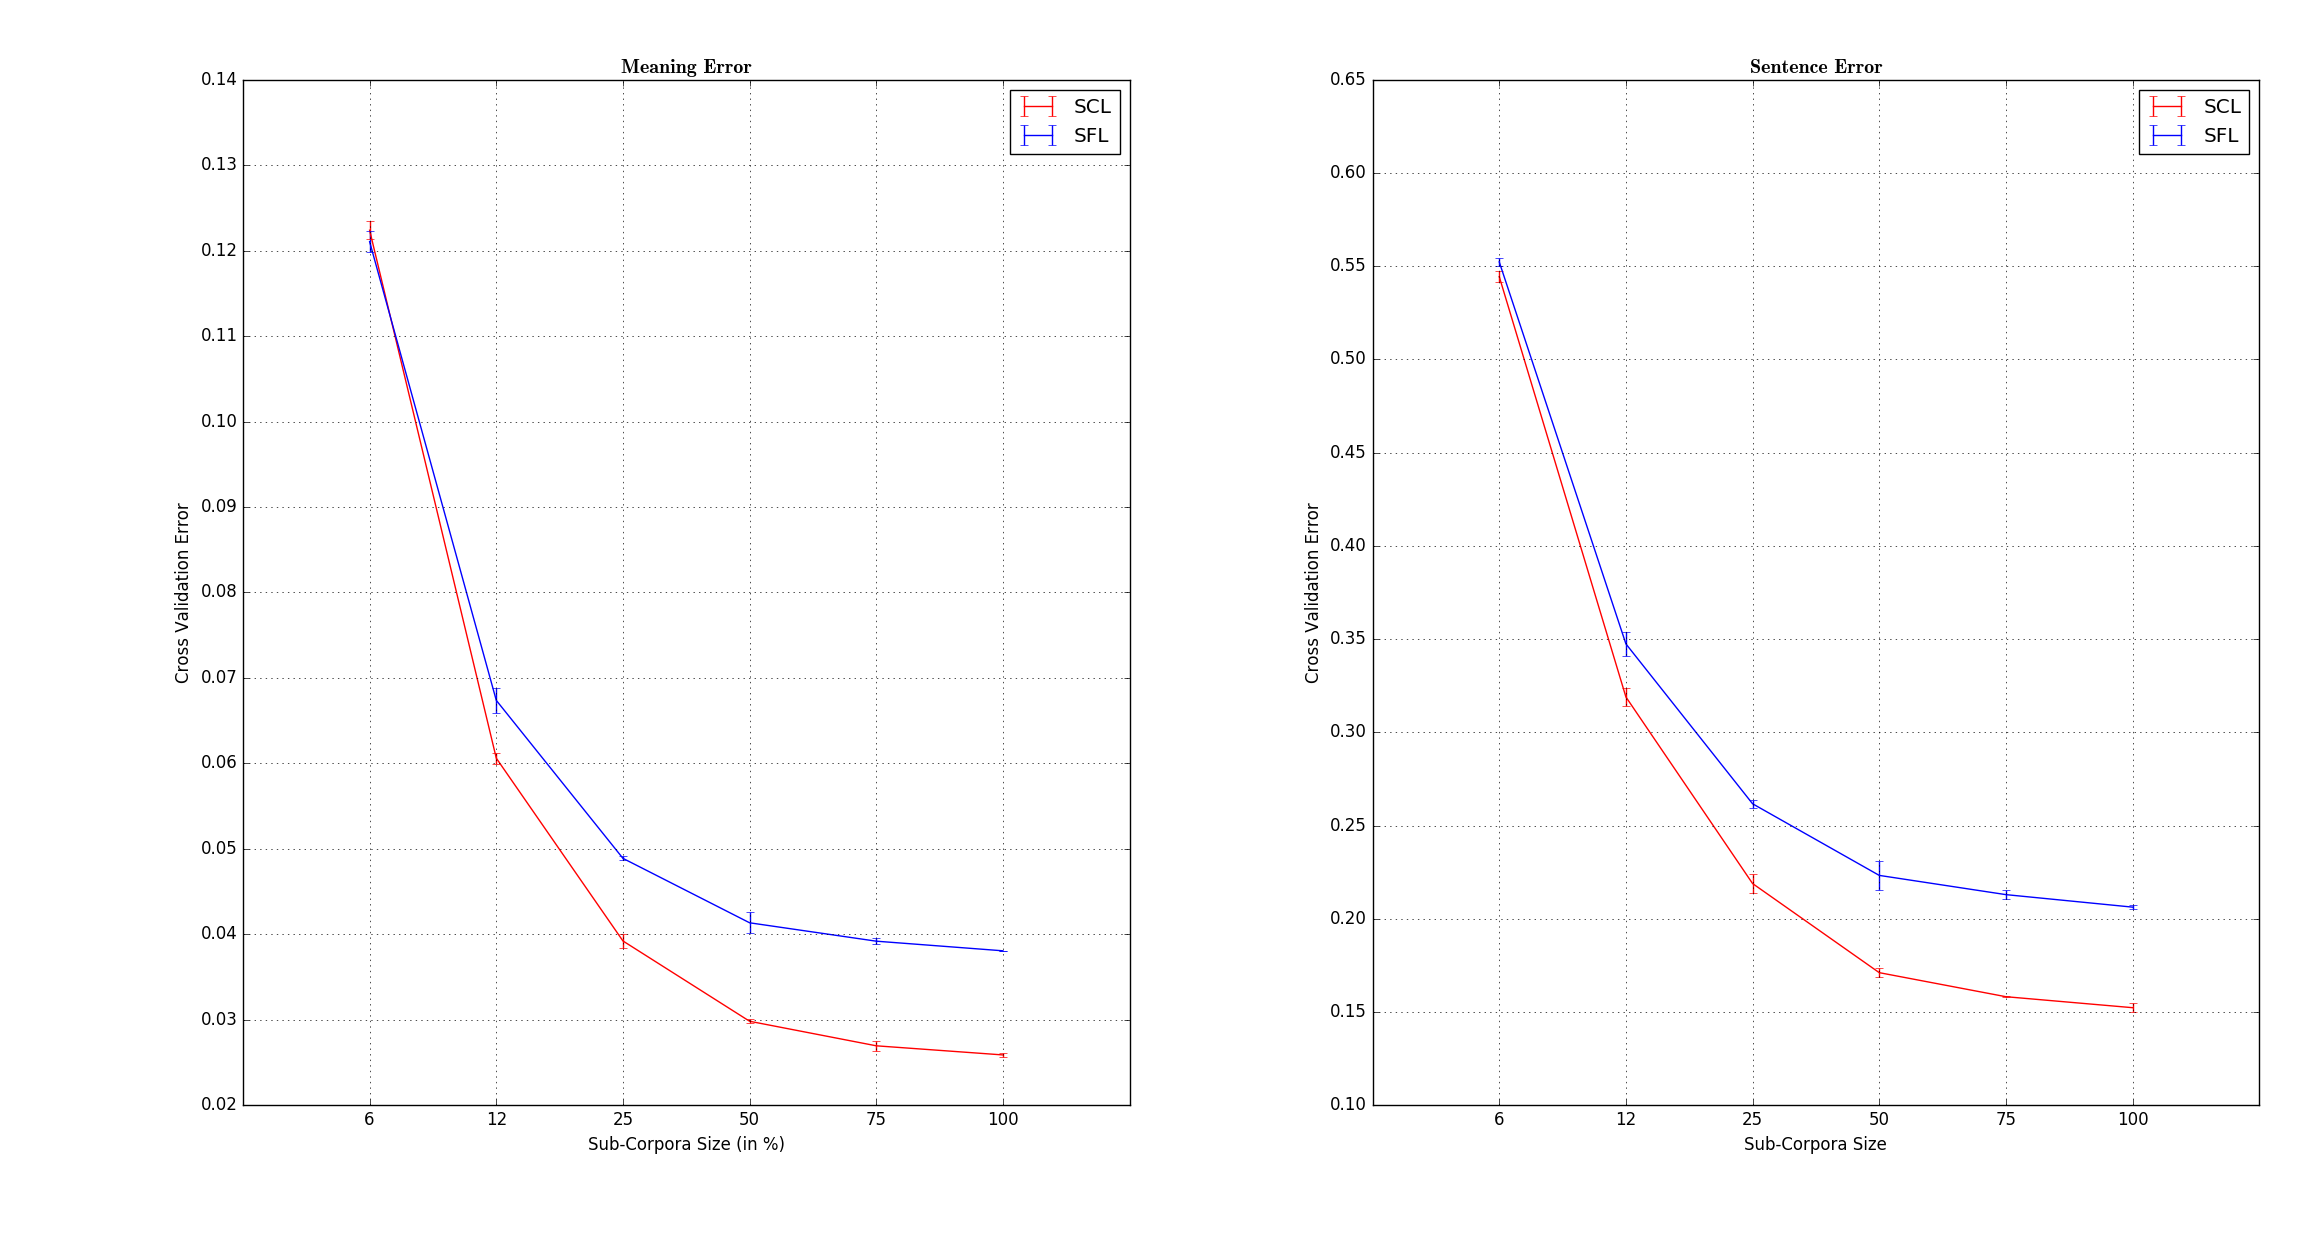
\includegraphics[width=1.0\linewidth]{corpus_size_1}
\caption[Effect of corpus size on Word2Vec-$\theta$RARes model]{\textbf{Effect of corpus size on cross validation errors of Word2Vec-SN model in SCL and SFL mode.} }
\label{fig:corpus_size_1}
\end{figure}

\begin{figure}[hbtp]
\centering
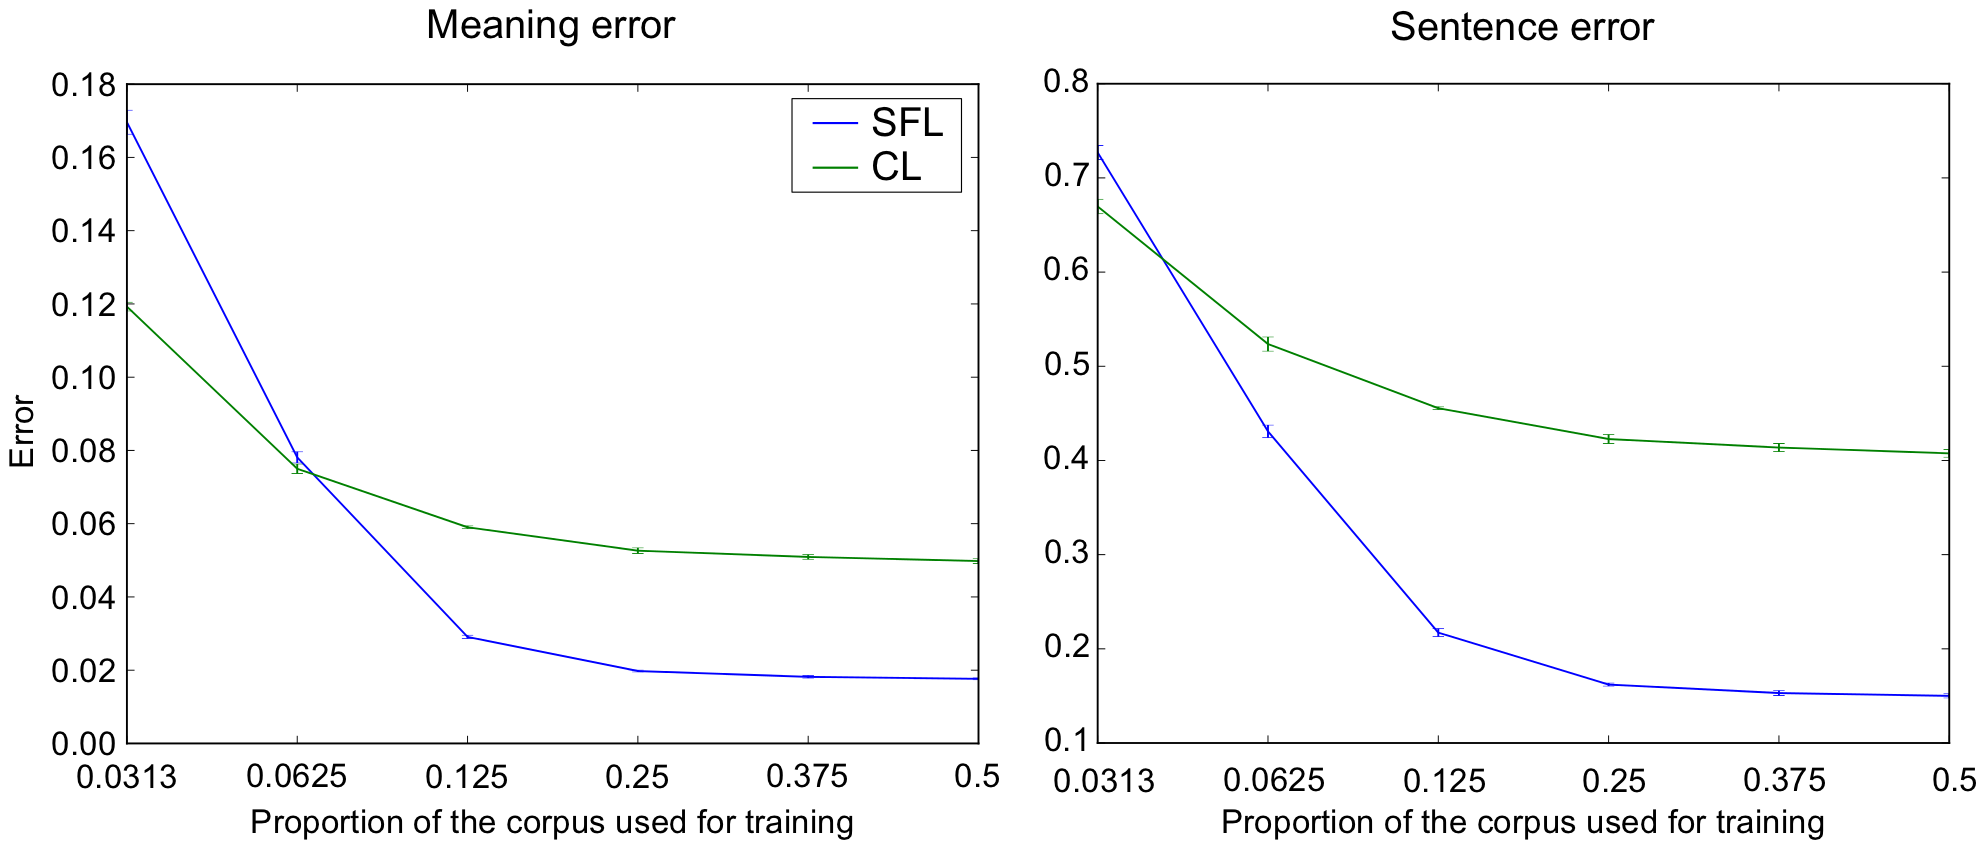
\includegraphics[width=1.0\linewidth]{corpus_size_xavier}
\caption[Effect of corpous size on Word2Vec-$\theta$RARes model]{Effect of corpus size on cross validation errors using $\theta$RARes model in SCL and SFL learning modes.}
\label{fig:corpus_size_xavier}
\end{figure}

Comparing the effect of corpus size on Word2Vec-$\theta$RARes model and the $\theta$RARes model (see fig. \ref{fig:corpus_size_xavier}), it was observed that in SFL mode, with increase in corpus size from $6\%$ to $25\%$, the meaning error in $\theta$RARes model dropped from $\approx 17\%$ to $\approx 4\%$ and sentence error dropped from $\approx 70\%$ to $\approx 20\%$. Whereas in the Word2Vec-$\theta$RARes model the meaning error dropped from $\approx 12\%$ to $\approx 5\%$  and the sentence error dropped from $\approx 55\%$ to $\approx 26\%$. Also, with the increase in corpus size further from $25 \%$ the cross-validation errors asymptotes in both the models with negligible improvement in error rates. Overall, the improvement in error rates with $\theta$RARes model in the SFL mode is higher as compared to Word2Vec-$\theta$RARes model.

Comparing the performance of both the models in the SCL mode, it can be seen that the meaning error in Word2Vec-$\theta$RARes model continuously drops when the corpus size is further increased from $12 \%$ whereas in the $\theta$RARes model the decline in meaning error is negligible. The sentence error in $\theta$RARes model, drops by a small amount when corpus size is increased from $6 \% $ to $25 \%$, but asymptotes as the corpus size is further increased from $25\%$ whereas it gradually drops in Word2Vec-$\theta$RARes model. From the lower to the upper limit of corpus size studied, it was observed that the sentence error in $\theta$RARes model dropped from $\approx 65\%$ to $\approx 40\%$ whereas in the Word2Vec-$\theta$RARes model it dropped from $\approx 55\%$ to $\approx 15 \% $. The meaning error, on the other hand, dropped from $\approx 12\%$ to $\approx 5\%$ in the $\theta$RARes model whereas, in the Word2Vec-$\theta$RARes model it dropped from $\approx 12\%$ to $\approx 2\%$.

Overall in SCL model it can be seen that on the range of sub-corpora size investigated in the experiment, the Word2Vec-$\theta$RARes model performed better than $\theta$RARes model with all sub-corpora sizes. Another pattern which can be observed is that with all sub-corpora sizes, the Word2Vec-$\theta$RARes model performs better in the SCL mode than the SFL mode. Whereas in the $\theta$RARes model, with the increase in corpus size the model performs better in SFL model than SCL mode. 

\section{Experiment-6: Generalization on new corpus}

Table \ref{tab:corpus_373} reports the mean sentence error and best generalization error values obtained with Word2Vec-$\theta$RARes and $\theta$RARes model. The best generalization error here represents the percentage of sentences whose meanings were predicted incorrectly in common within 10 model instances \cite{tra:xavier_hri}. The Word2Vec-$\theta$RARes model with a reservoir of 500 neurons, generalized with a sentence and best error of $42.65 \%$ and $26.54 \%$ respectively. Whereas with a reservoir of 1000 neurons, the Word2Vec-$\theta$RARes model generalized with $40.29 \%$ sentence and $25.73 \%$  best error. In comparison to the $\theta$RARes model, the mean sentence error in the Word2Vec-$\theta$RARes model improved by $26.31\%$ and $17.97\%$  with the reservoir of size 500 and 1000 respectively. The best generalization errors also improved by $17.96 \%$ and $9.12 \%$ with the reservoir size 500 and 1000 respectively.

The Word2Vec-$\theta$RARes model generalized better with both the reservoir sizes (500 and 1000) as compared to $\theta$RARes model. Notice the improvement in both the model with the increase in reservoir size from 500 to 1000 neurons. It can be seen that the improvement in cross-validation error in Word2Vec-$\theta$RARes model is comparatively less than $\theta$RARes model. The mean sentence error and best generalization error in $\theta$RARes improved by $10.7 \%$ and $9.65 \%$ respectively. Whereas with Word2Vec-$\theta$RARes model the mean sentence error and best generalization error improved by $2.36 \%$ and $0.81\%$ respectively with the increase in reservoir size from 500 to 1000 neurons.     

\begin{table}
\centering
\begin{threeparttable}
\caption[Word2Vec-$\theta$RARes model generalizing on new coprus]{Generalization error in SCL mode on corpus-373.}
\label{tab:corpus_373}
\rowcolors{2}{gray!25}{white}
\begin{tabularx}{\textwidth}{llYY}
\hiderowcolors
\toprule
Reservoir 	 		&  Error 	&   Word2Vec-$\theta$RARes Model		& $\theta$RARes Model \\
\midrule
\showrowcolors                 
\textbf{500 N}	& mean(std.) 		& 42.65 ($\pm$ 1.36) 	& 68.96 ($\pm$ 2.03)  \\
					& Best 			& 26.54 				& 44.50  \\
\textbf{1000 N}	& mean(std.) 		& 40.29 ($\pm$ 1.13) 	& 58.26 ($\pm$ 1.37)\\
					& Best 			& 25.73 				& 34.85 \\
\bottomrule
\end{tabularx}
\begin{tablenotes}
\small
\item 
Sentence and best errors (in $\%$) obtained with Word2Vec-$\theta$RARes model and $\theta$RARes in SCL mode with reservoir of size 500 and 1000 neurons. The results reported are mean and standard deviation of errors obtained from 10 reservoir instances. The best error here means the percentage of sentence errors common within all 10 reservoir instances \cite{tra:xavier_hri}.
\end{tablenotes}
\end{threeparttable}
\end{table}

Figure \ref{fig:373_stats_500} and \ref{fig:373_stats_1000} shows the number of erroneous sentences by number of model instances with reservoir size 500 and 1000 respectively. With a reservoir of 500 neurons (see fig. \ref{fig:373_stats_500}), all the ten instances of Word2Vec-$\theta$RARes and $\theta$RARes model correctly predicted the meaning of 146 and 35 sentences respectively. Whereas the meaning 99 and 166 sentences out of 373 were wrongly predicted by all the ten instances of Word2Vec-$\theta$RARes and $\theta$RARes model. 

With the increase in the reservoir from 500 to 1000 neurons, the number of sentences correctly predicted by all the model instances of Word2Vec-$\theta$RARes and $\theta$RARes model increased respectively from 146 to 160 and from 35 to 98. Also, the count of sentences where all model instances failed to predict the meaning correctly dropped from 99 to 96 and 166 to 130 for Word2Vec-$\theta$RARes model and $\theta$RARes model respectively. Notice that with both the reservoir sizes, the number of sentences whose meanings were correctly predicted by all the model instances of Word2Vec-$\theta$RARes model is higher than the $\theta$RARes model. Whereas the count of sentence wrongly predicted by all model instances are lower in Word2Vec-$\theta$RARes model as compared to that of $\theta$RARes model.

\begin{figure}[hbtp]
\centering
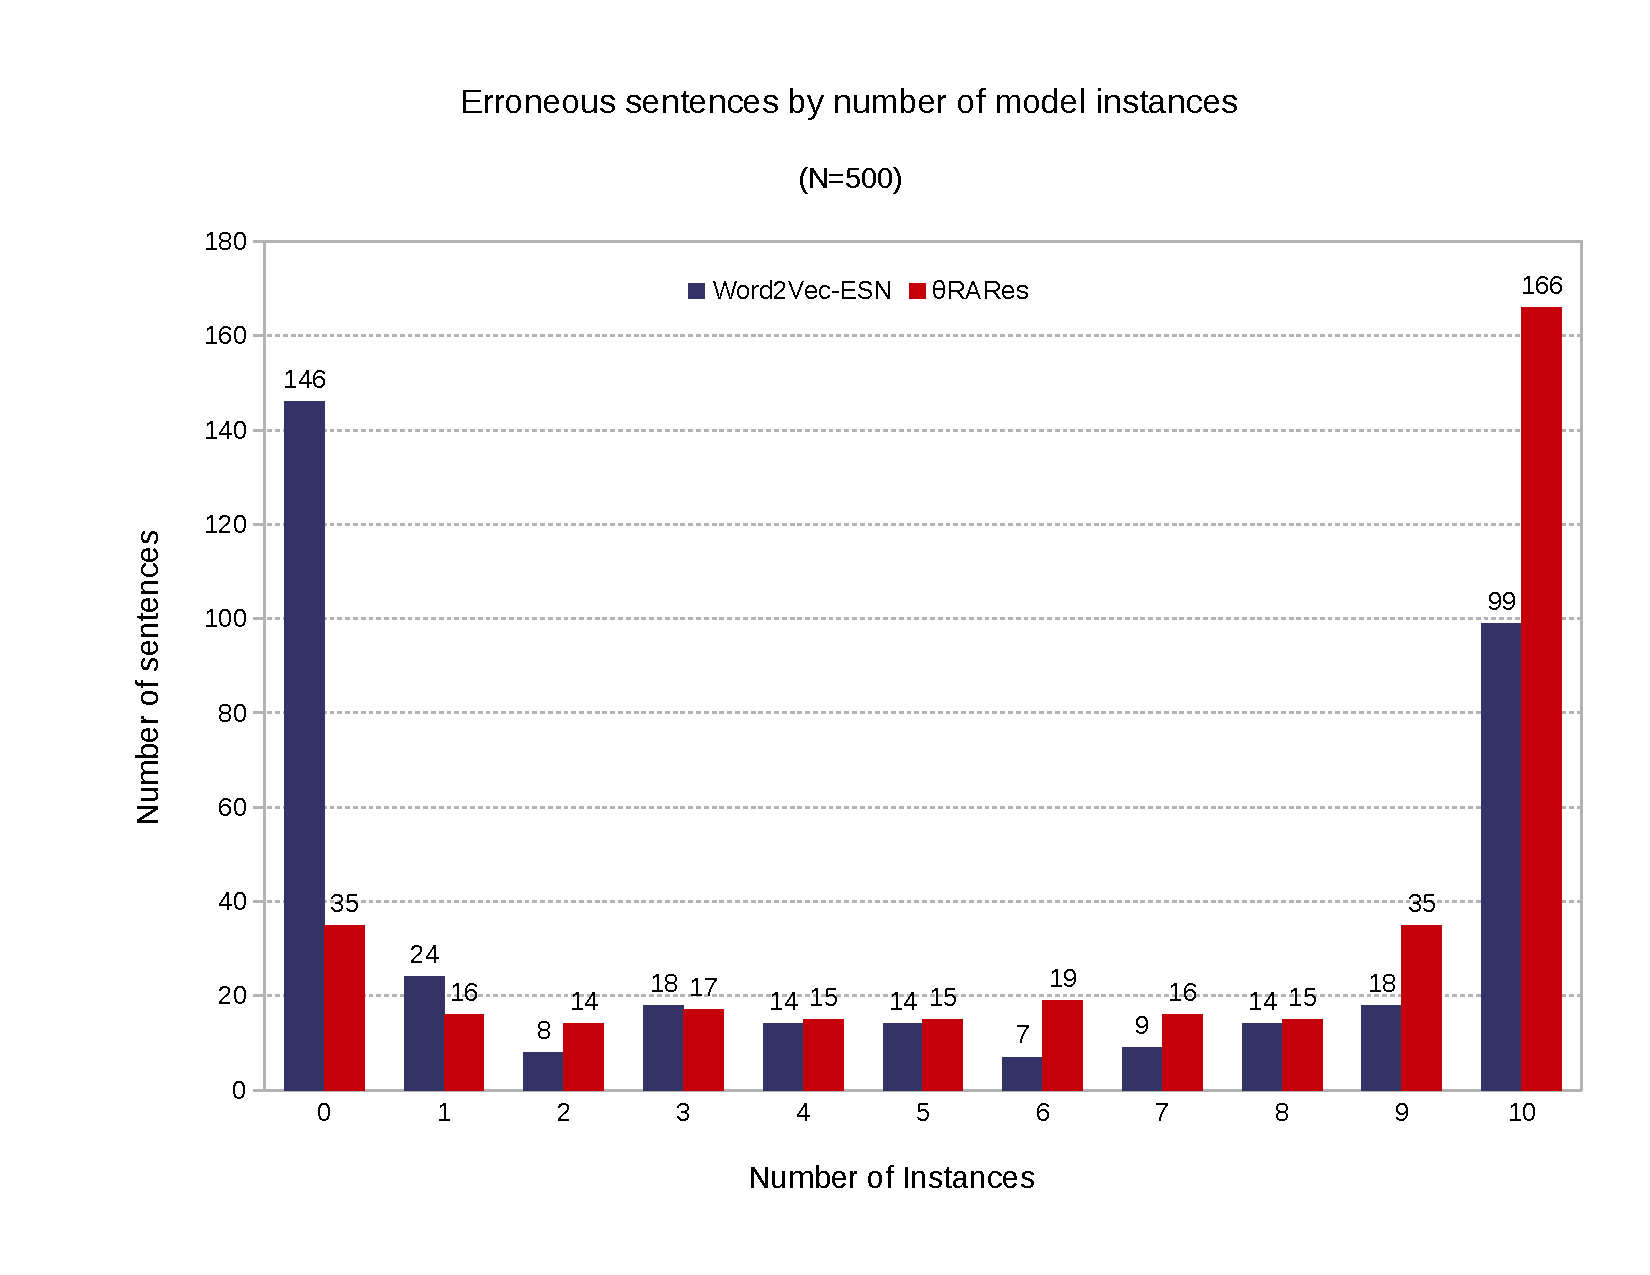
\includegraphics[width=0.9\linewidth]{500_res}
\caption[Sentence error count by number of instances with reservoir size 500]{Sentence error count by number of instances with reservoir of 500 neurons.}
\label{fig:373_stats_500}
\end{figure}

\begin{figure}[hbtp]
\centering
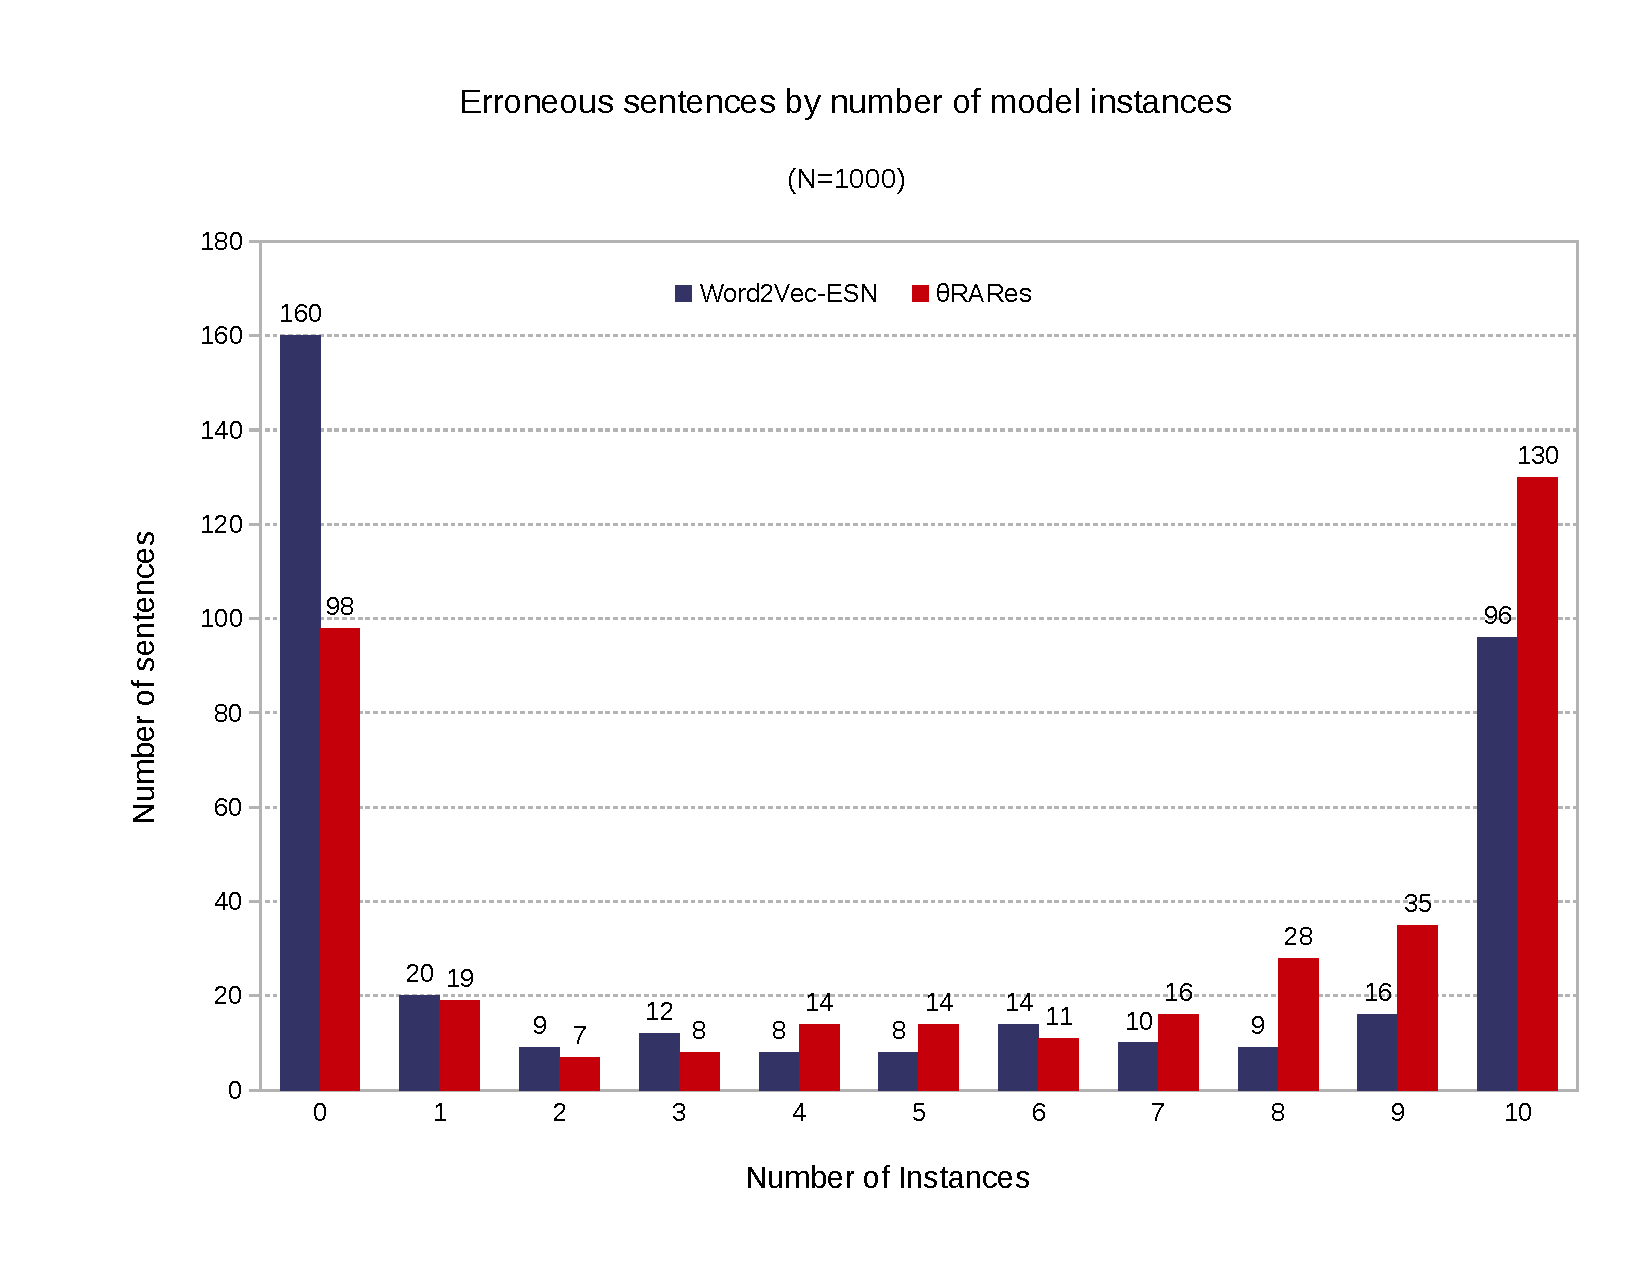
\includegraphics[width=0.9\linewidth]{1000_res}
\caption[Sentence error count by number of instances with reservoir size 1000]{Sentence error count by number of model instances with reservoir of 1000 neurons.}
\label{fig:373_stats_1000}
\end{figure}

\section{Experiment-7: Effect of Word2Vec word dimensions}

\paragraph{Word2Vec-$\theta$RARes model: } Figure \ref{fig:word_dim_scl} and \ref{fig:word_dim_sfl} shows the effect of word vector dimensions on cross-validation errors of Word2Vec-$\theta$RARes model in SCL and SFL mode respectively. The corresponding errors are also reported in Table \ref{tab:word-vector-size}. In the figures, we can see that from lower to the upper limit of the word vector dimensions studied, all the error measures in both the learning modes increased approximately by $2\%$. Also, in the range 20 to 200 dimensions, the cross-validation errors remained almost equivalent with negligible fluctuations. The minimum errors were obtained with word vectors of 30 dimensions i.e. $ME= 14.23$, $SE= 39.87$ in the SCL mode and  $ME= 16.61$, $SE= 43.46$ in the SFL mode. Another interesting pattern which can be observed is that with all the word vector dimensions the model in SCL mode always performed better as compared to SFL mode. The similar relation between SCL and SFL model was also observed in previous experiments as well. Overall we can say that the word vectors dimensions have a negligible effect on the performance of Word2Vec-$\theta$RARes model.

\begin{figure}[hbtp]
\centering
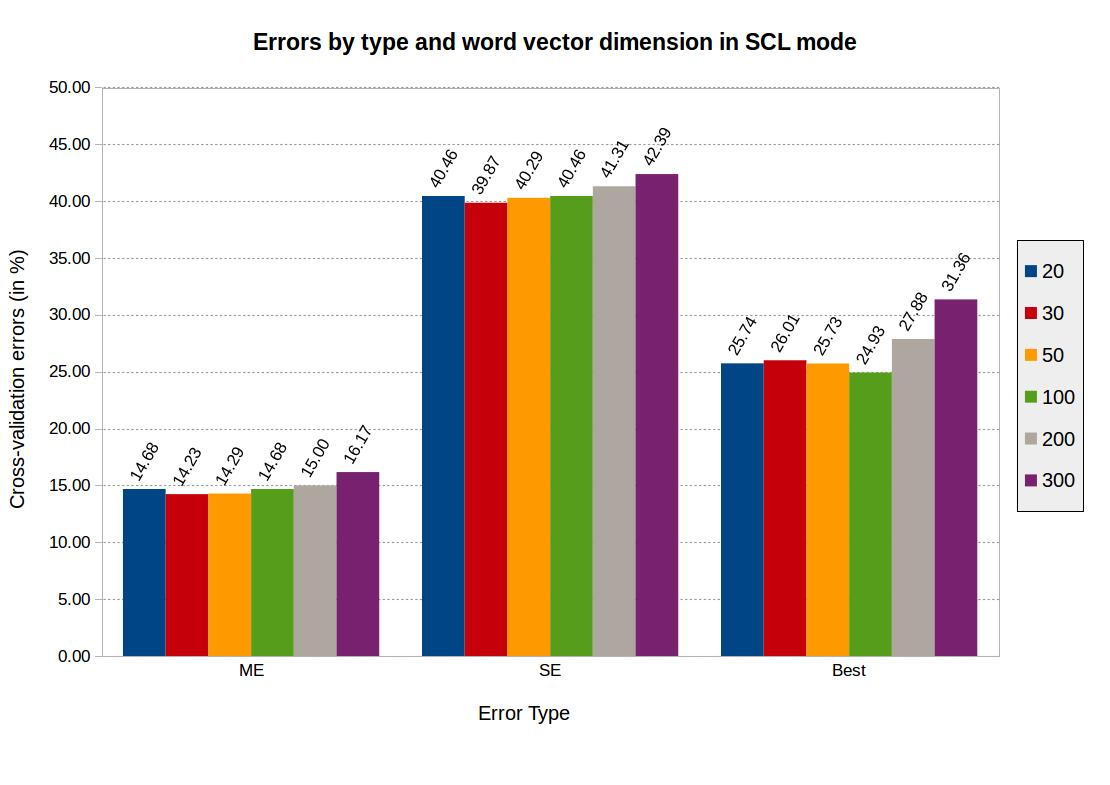
\includegraphics[width=0.9\linewidth]{word_dim_scl}
\caption[Effect of word vector dimensions on Word2Vec-$\theta$RARes model]{\textbf{Effect of word vector dimensions on cross validation errors of Word2Vec-$\theta$RARes model in SCL mode:} Cross-validation error are given in percentage. Error type includes ME: Meaning Error, SE: Sentence error, Best: Best generalization error.}
\label{fig:word_dim_scl}
\end{figure}

\begin{figure}[hbtp]
\centering
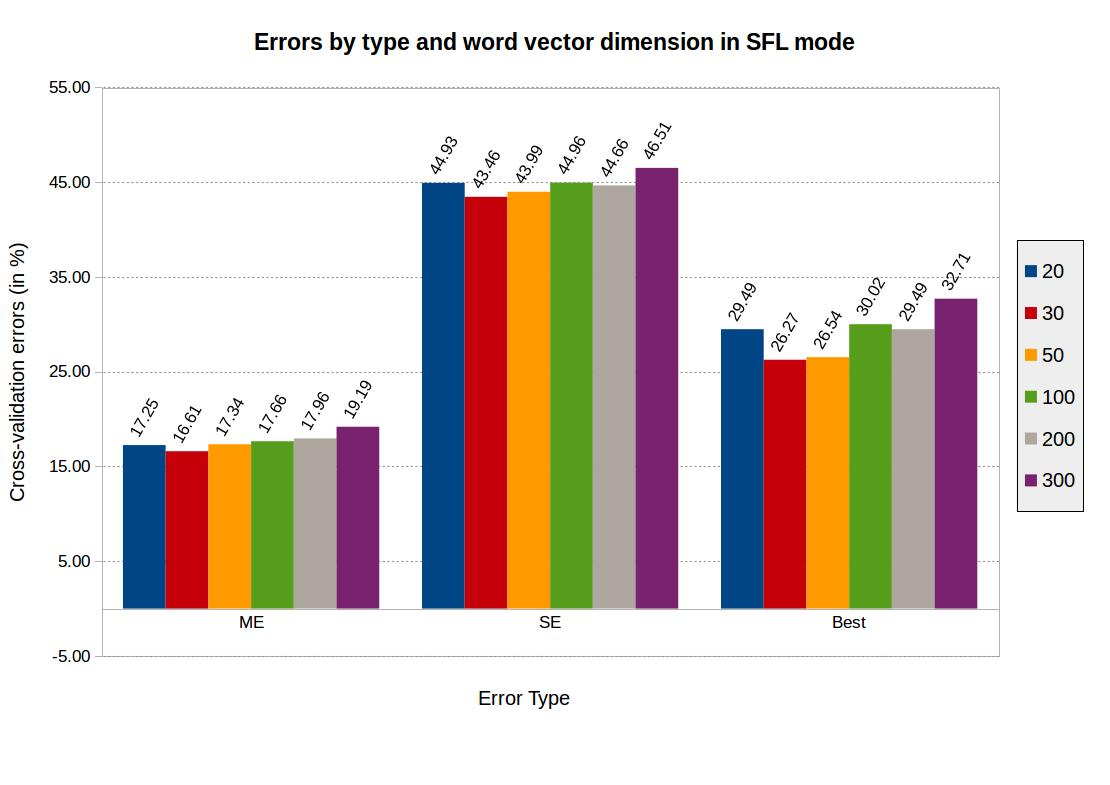
\includegraphics[width=0.9\linewidth]{word_dim_sfl}
\caption[Effect of word vector dimensions on Word2Vec-$\theta$RARes model]{\textbf{Effect of word vector dimensions on cross validation errors of Word2Vec-$\theta$RARes model in SFL mode:} Cross-validation errors are given in percentage. Error type includes ME: Meaning Error, SE: Sentence error, Best: Best generalization error.}
\label{fig:word_dim_sfl}
\end{figure}


\section{Neural output activity of the Word2Vec-$\theta$RARes model}

In the previous experiments, we observed that both the proposed model generalized well and the cross-validation error rates dropped with the increase in corpus size. So, the 45 sentences of corpus-45 were added to corpus-462 to get the resultant corpus have 507 sentences (462 + 45). The readout activations of the Word2Vec-$\theta$RARes model were then analyzed for the sentences in corpus-373 and newly formed coprus-507 to have the insight of how the system is processing the distributed word vectors to generate the meaning of the sentences. It was observed that the model is re-analyzing the thematic roles of input sentences across the time. The same behavior was also pointed out by Hinaut et. al \cite{tra:xavier_hri, xavier:2013:RT} with $\theta$RARes model.

\subsection{Output activity for the sentences with toplogically modified coded meaning}

Figure \ref{fig:act_analysis_1} shows the read out activations of the second noun in the following four sentences across time. Note that the sentences \ref{activation:sent-1} and \ref{activation:sent-2} with active constructions whereas \ref{activation:sent-3} and \ref{activation:sent-4} are passive constructions.

\begin{enumerate}[noitemsep]
\item the man \textit{gave}(V1) the \textit{book}(N2) to the boy. \label{activation:sent-1}
\item the man \textit{took}(V1) the \textit{ball}(N2) that \textit{hit}(V2) the glass. \label{activation:sent-2}
\item the boy \textit{caught}(V1) the \textit{ball}(N2) that was \textit{thrown}(V2) by the man.  \label{activation:sent-3} 
\item the ball was \textit{pushed}(V1) by the \textit{man}(N2).  \label{activation:sent-4}
\end{enumerate}

Each colored lines in the graph represent the possible thematic roles of the second noun (N2) which can have one of the three possible roles i.e. Agent (A), Object (O) or Recipient (R) with respect to either Verb-1 (V1) or Verb-2 (V2). N2 is marked in red and verbs are marked in green on the x-axis. In the figure the role `N2-A-V1' can be interpreted as the second noun (N2) is the agent of first verb (V1).. 

As all the four sentences start with `the', activations at this word is same for all four sentences. With the introduction of the first noun (`man') in sentences \ref{activation:sent-1} and \ref{activation:sent-2}, the readout activations of role N2 as object of V1 (N2-O-V1) goes above the threshold 0. Thus the model predicts that the N2 could be the object of V1. In sentence \ref{activation:sent-3}, with the arrival of the first noun (`boy'), the competition between roles N2-A-V1, N2-A-V2, and N2-O-V2 can be seen, but only the role N2-A-V1 (agent of verb caught) managed to cross the threshold. Whereas, in sentence \ref{activation:sent-4}, the activation of role with N2-A-V1 is higher when the first noun (`ball') is encountered, but with the arrival `was' the role of N2 is changed as recipient of V1 (`pushed').

In sentence \ref{activation:sent-2}, with the advent of the V1 (`took') the activation for N2-A-V2 goes above threshold indicating the presence of V2 (`hit') in the sentence even before the model has encountered the second verb. Whereas in sentence \ref{activation:sent-1}, the activation of role N2-A-V1 maintained and no other role managed to cross the threshold with the arrival of V1 (`gave'). In sentence \ref{activation:sent-3} and \ref{activation:sent-4}, with the arrival of V1 (`caught' and `pushed' respectively) one can notice the re-analysis made by the model. In sentence \ref{activation:sent-3}, the activation of N2-A-V1 goes below the threshold and takes the new role as the object of both V1 and V2 i.e. N2-O-V1 and N2-O-V2. In sentence \ref{activation:sent-4}, the previously predicted role N2-R-V1 goes below threshold with the arrival of V1 (`pushed').

Throughout the rest of sentence \ref{activation:sent-1}, the prediction N2-O-V1 is maintained with some minor ups and downs. In sentence \ref{activation:sent-2}, the predictions of N2 alternates between O-V1 and A-V2 where the arrival of "the ball" seems to favor O-V1, the arrival of "that" changes the prediction again to A-V2. In both cases, the activation of both the role 0-V1 and A-V2 remains above the threshold. In sentence \ref{activation:sent-3} the model sees both O-V1 and R-V1 as the preferred predictions, both being almost with similar activations and only alternating slightly. In sentence \ref{activation:sent-4}, the prediction of role N2 as agent of V1 do not change again throughout the sentence ever since arrival of V1 (`pushed').

\begin{figure}[hbtp]
\centering
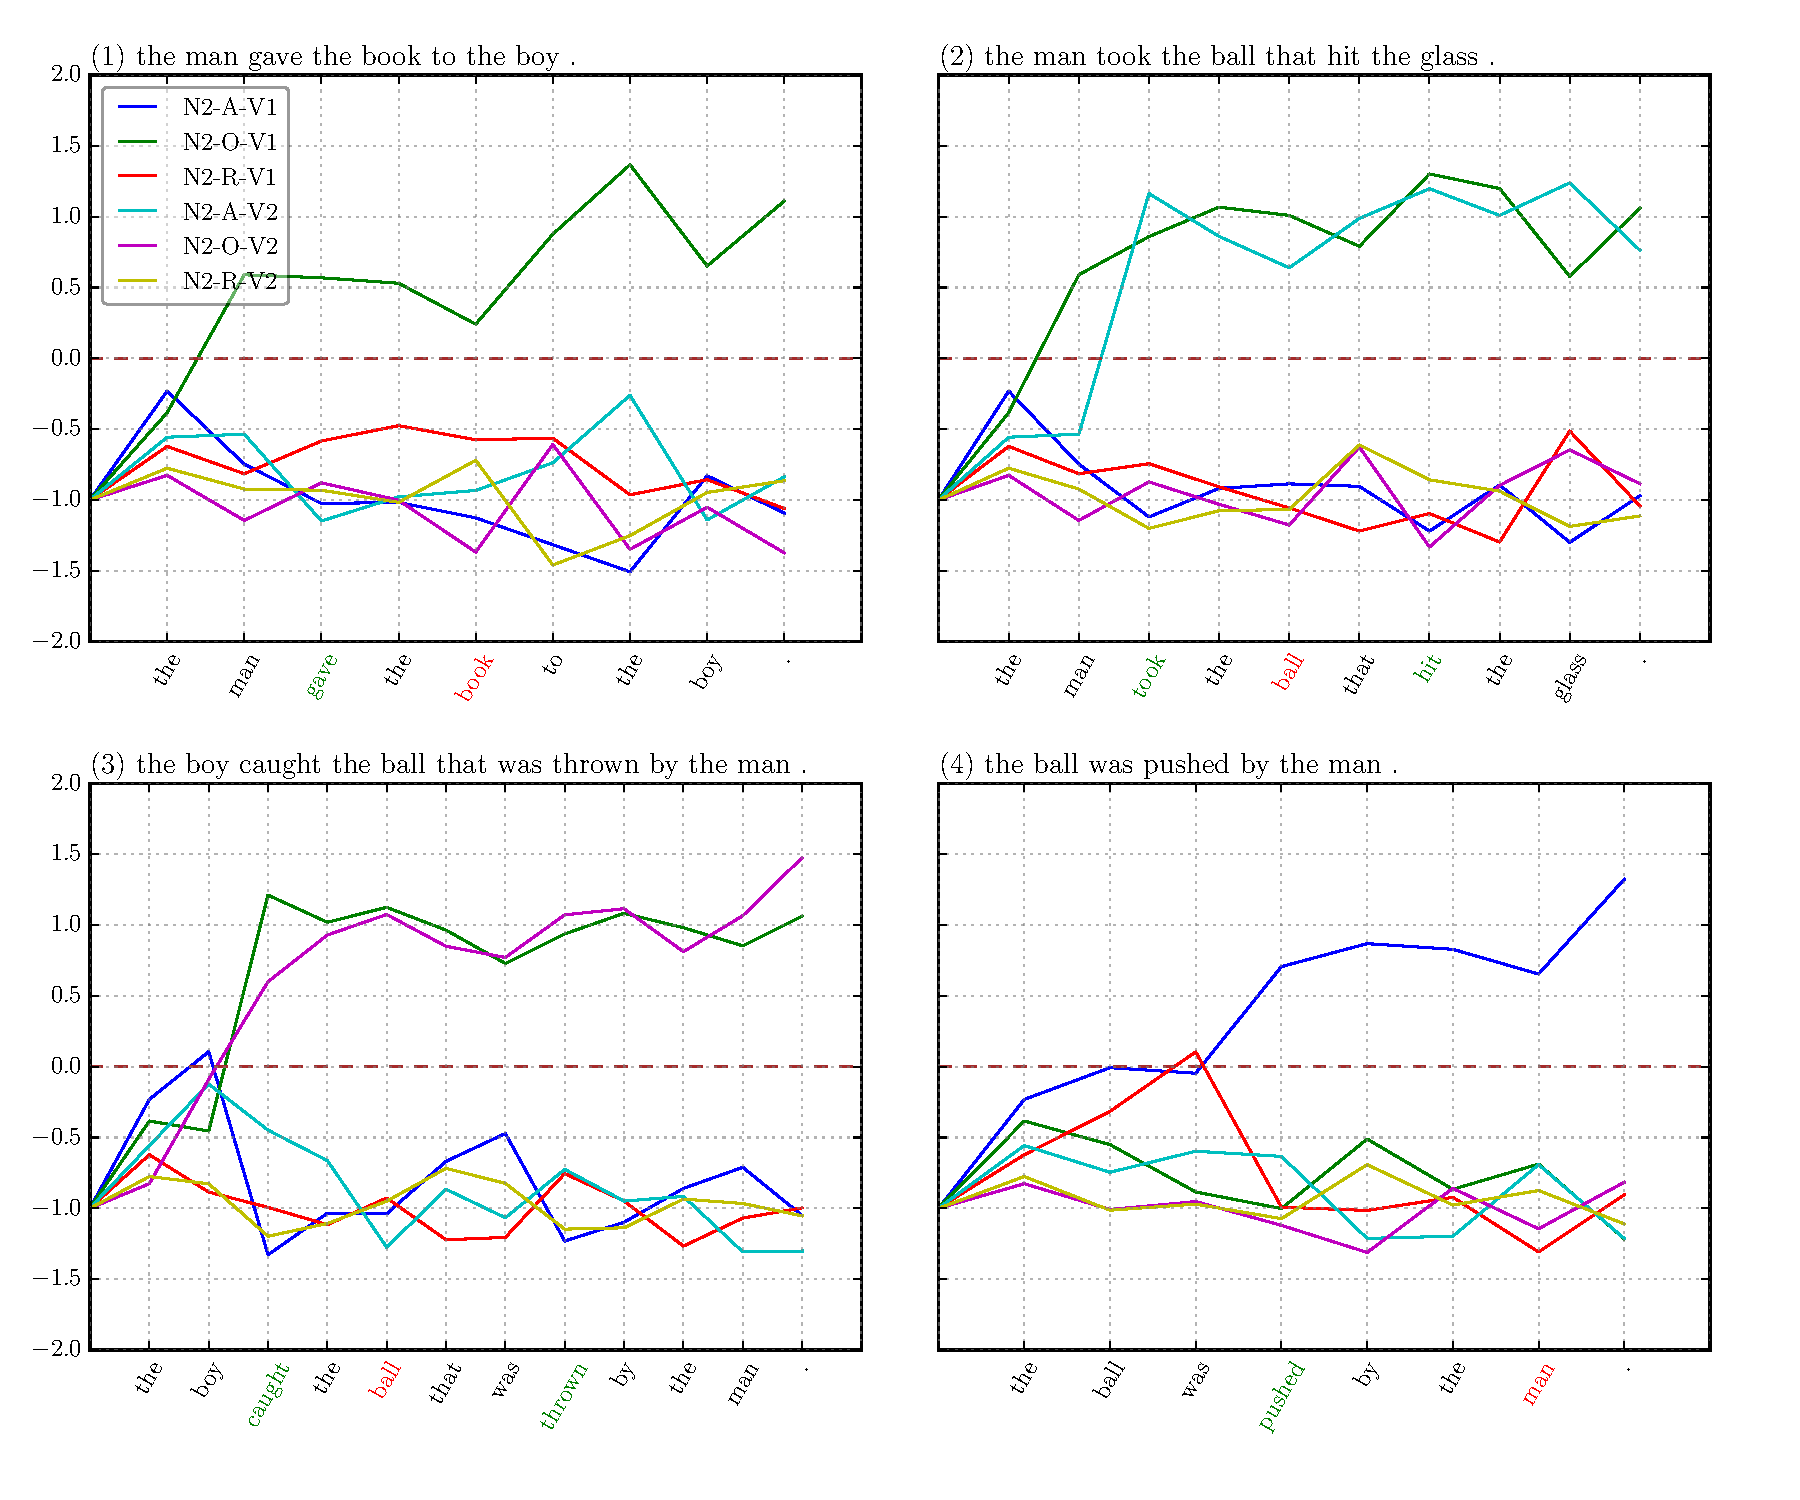
\includegraphics[width=1.0\linewidth]{act_analysis_1}
\caption[Online re-analysis of activation by Word2Vec-$\theta$RARes Language model:]{\textbf{Online re-analysis of activation by Word2Vec-$\theta$RARes Language model:} Each coloured line shows the thematic role of Noun-2 (tick marked in red) with respect to Verb-1 and Verb-2 (ticks shown in green).}
\label{fig:act_analysis_1}
\end{figure}

\begin{figure}[hbtp]
\centering
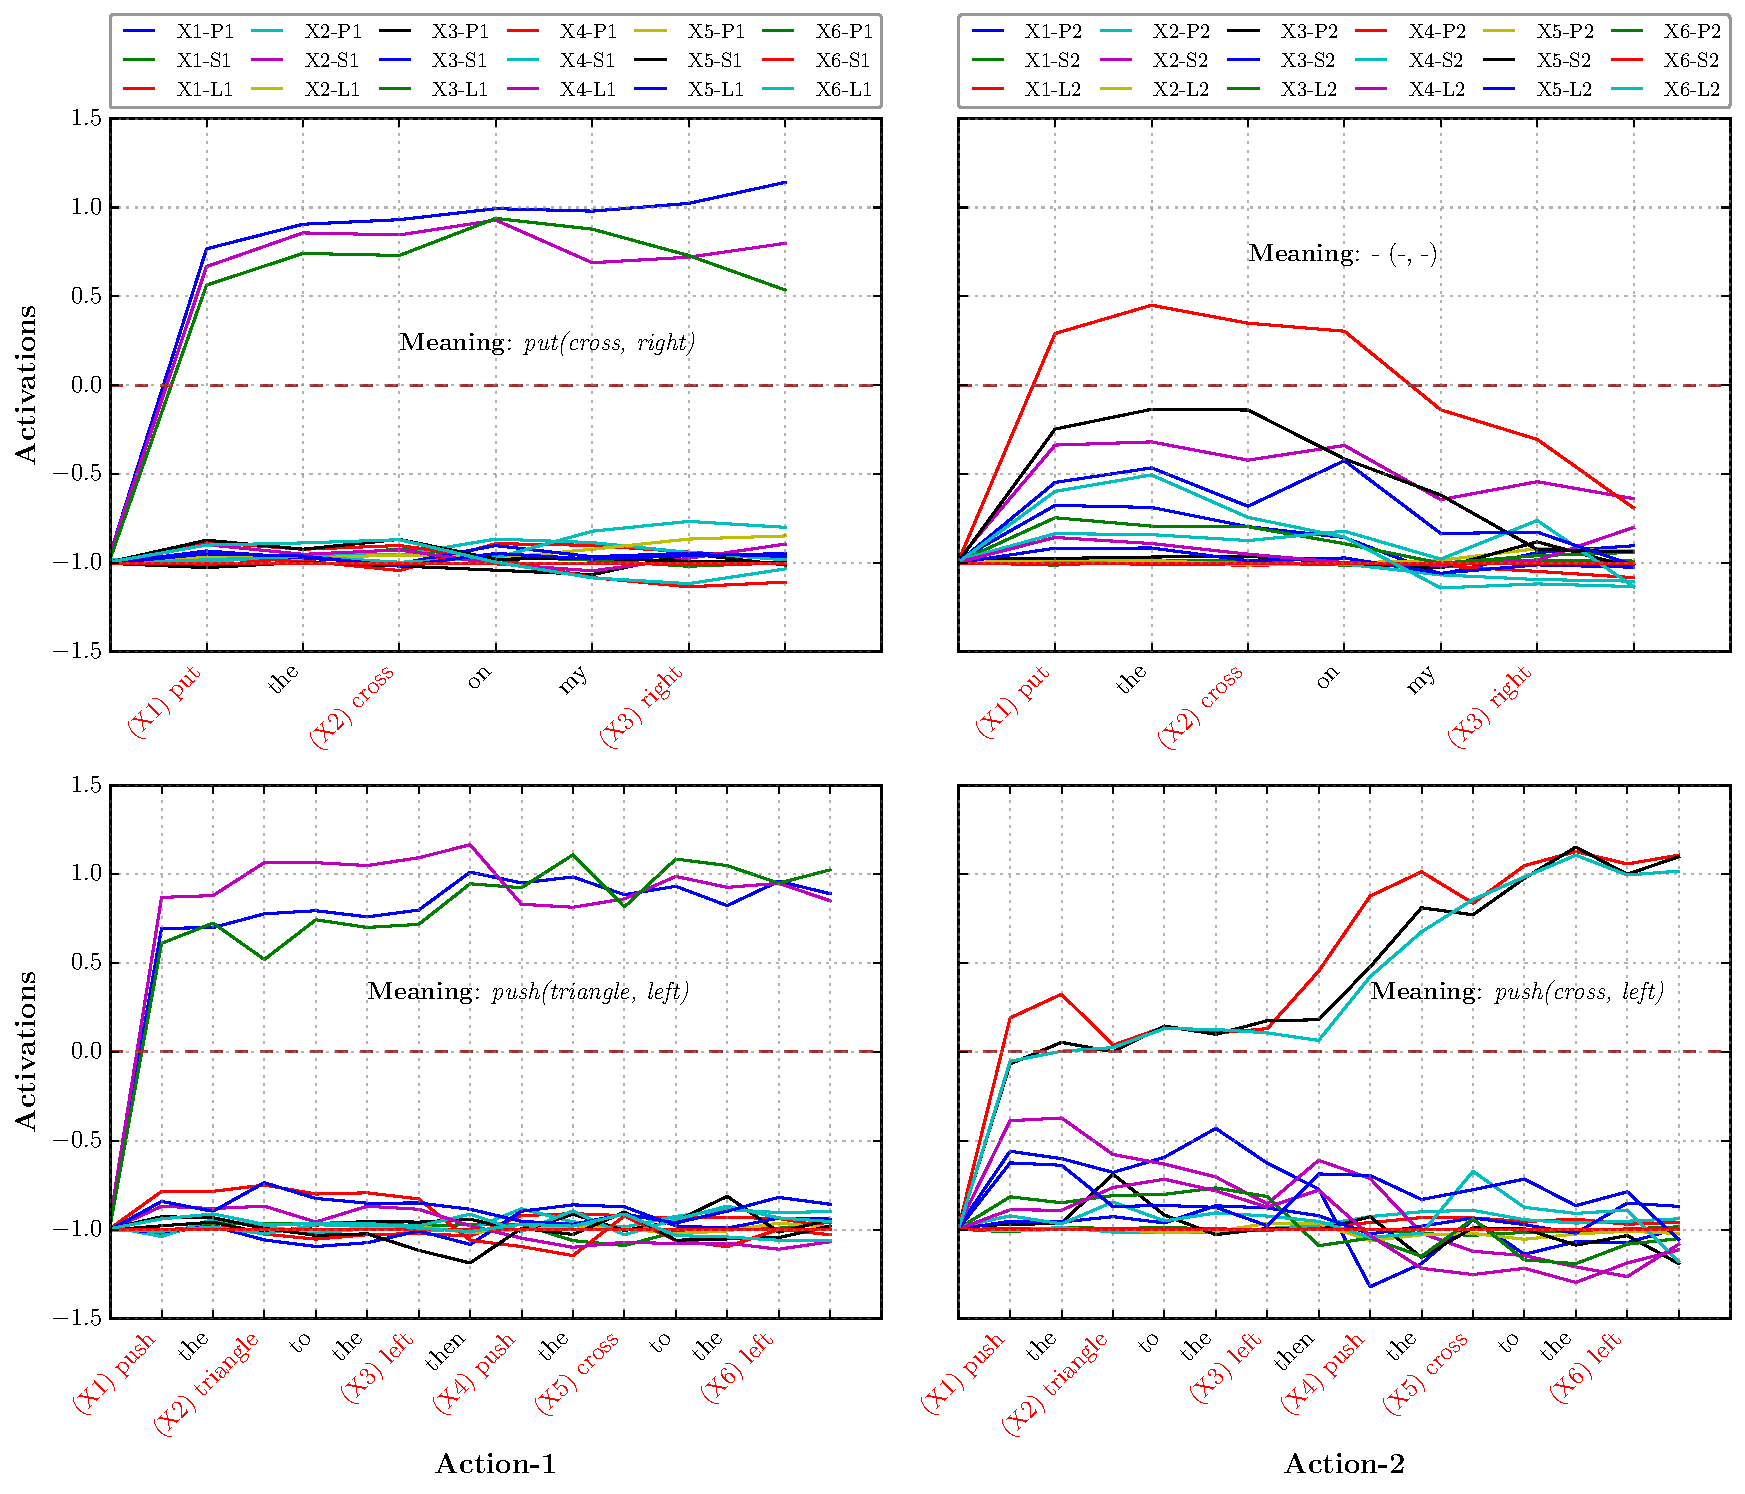
\includegraphics[width=1.0\linewidth]{act_analysis_2}
\caption[Readout activity of Word2Vec-$\theta$RARes model for a simple and complex sentence from corpus-373]{\textbf{Readout activity of Word2Vec-$\theta$RARes model for a simple and complex sentence from corpus-373:} }
\label{fig:act_analysis_2}
\end{figure}

\subsubsection{Output activity for sentences without toplogically modified coded meaning} 

Figure \ref{fig:act_analysis_2} shows the readout activations of the following two sentences for action-1 and action-2. 

\begin{enumerate}[noitemsep,label=(\Alph*) ]
\item \textit{put}(X1) the \textit{cross}(X2) on my \textit{right}(X3) \label{activation:sent-a}
\item \textit{push}(X1) the \textit{triangle}(X2) to the \textit{left}(X3) then \textit{push}(X4) the \textit{cross}(X5) to the \textit{left}(X6) \label{activation:sent-b}
\end{enumerate}

Note that the sentence \ref{activation:sent-a} is a simple sentence with only one action and three semantic words (X1-X3), whereas sentence \ref{activation:sent-b}, is a complex sentence with two actions and six semantic words (X1-X6). Each semantic word in the sentences can have a role with respect to an action. A role X1-P1, for example, is interpreted as the first semantic word (X1)  is the predicate of action-1. The roles predicate, subject and location are represented by `P', `S' and `L' respectively.

In the first row of Figure \ref{fig:act_analysis_2}, the readout activity of the model for sentence \ref{activation:sent-a} is shown for each action (2 actions in our case). One can see that for action-1, the model correctly predicts the meaning \textit{put(cross, right)}, whereas for the action-2, at the end of sentence all the neural activations go below the threshold 0. Thus, this indicates the presence of only action-1 in the sentence. Also notice the online re-analysis behavior of the model, where for the action-2, the activation of role (X1-L2) goes above threshold 0 at the beginning of the sentence but later drop below 0 at the end of the sentence.

The second row of Figure \ref{fig:act_analysis_2}, illustrate the readout activity of sentence \ref{activation:sent-b} for each action. The model correctly predicts the thematic roles of constituent semantic words (X1 to X6) for both the actions. For the action-1 the model makes early predictions of roles i.e. \textit{push (triangle, left)}, whereas, for action-2, the activation of correct roles are reinforced when the model encounters the second predicate (X4 = `push') in the sentence. Thus the model predicts the meaning of sentence for the second action as \textit{push (cross, left)}.

\section{Evaluating Word2Vec-$\theta$RARes model performance}

In the previous section, we saw the online re-analysis of sentence meanings by Word2Vec-$\theta$RARes model. Previously, we also saw the performance of Word2Vec-$\theta$RARes model in numbers. In this section, we will see that for what type of the sentences the proposed model performed better than $\theta$RARes model on TRA task and vice-versa. This analysis was done on results obtained in Experiment-6 using corpus-373.

While analyzing the sentences whose meanings were correctly predicted by all ten instances of Word2Vec-$\theta$RARes model and incorrectly predicted by $\theta$RARes model, a significant pattern was identified. Almost $85 \%$ of the sentences wrongly predicted by all instances of $\theta$RARes model were either two action commands or redundant commands (see fig. \ref{fig:meaning_realtions}). For example ``push the circle in the middle and put it in the right" and ``push the circle to the middle and then put it on the right".

Table \ref{tab:color_error} and Table \ref{tab:anaphoric_error}, reports the sentences whose meanings were predicted wrongly at least by one instance of $\theta$RARes model and correctly predicted by all the instances of the Word2Vec-$\theta$RARes model. It was observed $\theta$RARes model failed to predict the meaning of most of the sentences in which the color of the objects to be moved is specified. In other words, the model failed to predict the meaning os sentences where of adjectives like \textit{`red'} or \textit{`blue'} are used with semantic words (see table \ref{tab:color_error}).  Similarly, sentences in Table\ref{tab:anaphoric_error}, includes anaphoric reference word \textit{`it'} (sentences 1-3), pointing to a semantic word within the discourse of sentence . Also, there are instructions which specify an action to be repeated using the anaphoric words `twice' or `two times' (sentences 4-7). Such sentences were also predicted incorrectly by at least one instance of $\theta$RARes model. Whereas, the proposed Word2Vec-$\theta$RARes model, correctly predicts the meanings these sentences. $\theta$RARes model also failed to predict the meaning of sentences where the reference location was given with respect to the person instructing the robot (sentences 1, 8, 9), whereas Word2Vec-$\theta$RARes model predicted them correctly. 

% Please add the following required packages to your document preamble:
\begin{table}[H]
\centering
\caption{Example sentences correctly predicted by all 10 instances of Word2Vec-$\theta$RARes model and mispredicted atleast once with $\theta$RARes model. }
\label{tab:color_error}
\resizebox{\textwidth}{!}{%
\begin{tabular}{|c|l|l|l|}
\hline
\multicolumn{1}{|c}{\multirow{2}{*}{\textbf{S.No}}} & \multicolumn{1}{|c|}{\multirow{2}{*}{\textbf{Sentences}}} & \multicolumn{2}{c|}{\textbf{\begin{tabular}[c]{@{}c@{}}Actual  Meaning\\ Predicate(Object,Location)\end{tabular}}} \\ \cline{3-4} 
\multicolumn{1}{|c}{} & \multicolumn{1}{|c|}{} & \multicolumn{1}{c|}{\textit{\textbf{Action-1}}}& \multicolumn{1}{c|}{\textit{\textbf{Action-2}}}         \\ \hline

1&point the red cross and point the circle                           & point(cross, -) 		& point(circle, -) 	\\ \hline
2&put the red cross to the left and hit the blue circle              & put(cross, left)		& hit(circle, -) 	\\ \hline
3&grasp the red cross and then point the circle                      & grasp(cross, - )		& point(circle, -) 	\\ \hline
4&after putting the red cross to the left please hit the blue circle & putting(cross, left)	& hit(circle, -) 	\\ \hline
5&please grasp the red cross										   & grasp(cross, -) 		&	-				\\ \hline
\end{tabular}%
}
\end{table} 

% Please add the following required packages to your document preamble:
\begin{table}[H]
\centering
\caption{My caption}
\label{tab:anaphoric_error}
\resizebox{\textwidth}{!}{%
\begin{tabular}{|c|l|l|l|}
\hline
\multicolumn{1}{|c}{\multirow{2}{*}{\textbf{S.No}}} & \multicolumn{1}{|c|}{\multirow{2}{*}{\textbf{Sentences}}} & \multicolumn{2}{c|}{\textbf{\begin{tabular}[c]{@{}c@{}}Actual  Meaning\\ Predicate(Object,Location)\end{tabular}}} \\ \cline{3-4} 
\multicolumn{1}{|c}{} & \multicolumn{1}{|c|}{} & \multicolumn{1}{c|}{\textit{\textbf{Action-1}}} & \multicolumn{1}{c|}{\textit{\textbf{Action-2}}}  \\ \hline

1&before grasping the triangle on my left point at it.     & point (triangle, -)  & grasping(triangle,-)   \\ \hline
2&before grasping the triangle point at it.                & point (triangle, -)  & grasping(triangle,-)   \\ \hline
3&before hitting the triangle point at it.                 & point (triangle, -)  & hitting (triangle,-)   \\ \hline
4&grasp circle two times 									& grasp(circle, -) 		& grasp(circle, -) 		 \\ \hline
5&point cross two times 									& point(cross,-) 		& point(cross, -)		 \\ \hline
6&hit twice the blue circle 								& hit(circle, -) 		& hit(circle, -)		 \\ \hline
7&grasp the circle twice 									& grasp(circle,-) 		& grasp(circle, -)	   	\\ \hline
8&point the circle on my left                              & point (circle, -)    & -						\\ \hline
9&push the cross on my left and then grasp the circle      & push (cross, left)   & grasp (circle, -)     \\ \hline
\end{tabular}%
}
\end{table} 

So far, we have seen the upside of Word2Vec-$\theta$RARes model over $\theta$RARes model, but there are cases where Word2Vec-$\theta$RARes model fails as well and are reported in Table \ref{tab:common_error}. It was observed that in most of the cases, the meaning of the sentences with complex structures where the first action to be performed is specified after the second action, using words `after having' are predicted wrongly by both the models (sentences 2-4 ). Also, the Word2Vec-$\theta$RARes model fails to predict the meaning of grammatically incorrect sentences in most of the cases e.g. sentence 1. It was also noticed that use of word contractions e.g. `youve', `weve' etc. in the sentences also leads to an error in meaning prediction by Word2Vec ESN model.

\begin{table}[h]
\centering
\caption{My caption}
\label{tab:common_error}
\resizebox{\textwidth}{!}{%
\begin{tabular}{|c|l|l|l|}
\hline
\multicolumn{1}{|c}{\multirow{2}{*}{\textbf{Sentences}}} & \multicolumn{1}{|c|}{\multirow{2}{*}{\textbf{Sentences}}} & \multicolumn{2}{c|}{\textbf{\begin{tabular}[c]{@{}c@{}}Actual  Meaning\\ Predicate(Object,Location)\end{tabular}}} \\ \cline{3-4} 
\multicolumn{1}{|c}{} & \multicolumn{1}{|c|}{} & \multicolumn{1}{c|}{\textit{\textbf{Action-1}}} & \multicolumn{1}{c|}{\textit{\textbf{Action-2}}} \\ \hline

1&in left push the triangle and the cross                  & push(triangle, left )   & push(cross, left)  \\ \hline
2&grasp the circle but before put the cross on the left    & put(cross, left )        & grasp(circle,-)    \\ \hline
3&touch the cross after having touch the triangle          & touch(triangle,-)        & touch(cross,-)     \\ \hline
4&put the triangle to the left after having touched it     & touched (triangle,-)     & put triangle left   \\ \hline
5&touch the circle after youve pointed the triangle        & pointed(triangle,-)      & touch(circle,-)    \\ \hline
6&put the cross over to the left and then once youve & & \\ &done that grasp the circle   & put(cross, left ) & grasp(circle,-) \\ \hline

\end{tabular}
}
\end{table}














 






















